\documentclass[a4paper]{article}
\usepackage[left=2cm, right=2cm,bottom=2cm]{geometry}
\usepackage{lipsum}
\usepackage{tikzpagenodes}
\usepackage{pgfplots}
\usepackage{tikz}
\usepackage{tikz-3dplot}
\usetikzlibrary{arrows,decorations.pathmorphing,backgrounds,positioning,fit,matrix}
\pgfplotsset{compat=1.8}
\usepackage{graphics} % for pdf, bitmapped graphics files
\usepackage{epsfig} % for postscript graphics files
\usepackage[colorlinks=true,citecolor=green]{hyperref}
\usepackage{cite}
\usepackage{amsmath,amssymb,amsfonts}
\usepackage{algorithmic}
\usepackage{graphicx}
\usepackage{url}
\usepackage{cite}
\usepackage{bm}
\usepackage{pbox}
\usepackage{siunitx,booktabs,etoolbox}
\usepackage{ulem}
\usepackage{titling}
\usepackage{float}
%\usepackage{pgf,tikz,pgfplots}
%\pgfplotsset{compat=1.15}
%\usepackage{mathrsfs}

\usetikzlibrary{arrows}

\def\BibTeX{{\rm B\kern-.05em{\sc i\kern-.025em b}\kern-.08em
		T\kern-.1667em\lower.7ex\hbox{E}\kern-.125emX}}
\title{Ex3: MRF, Deformable Models \& Geometric Priors}
\author{Xiao Hu, emails: \url{xiahaa@space.dtu.dk}}
\begin{document}
	\maketitle
	\thispagestyle{empty}
	\section{Feed Forward Neural Network}
	\begin{figure*}[htbp]
	\centering
	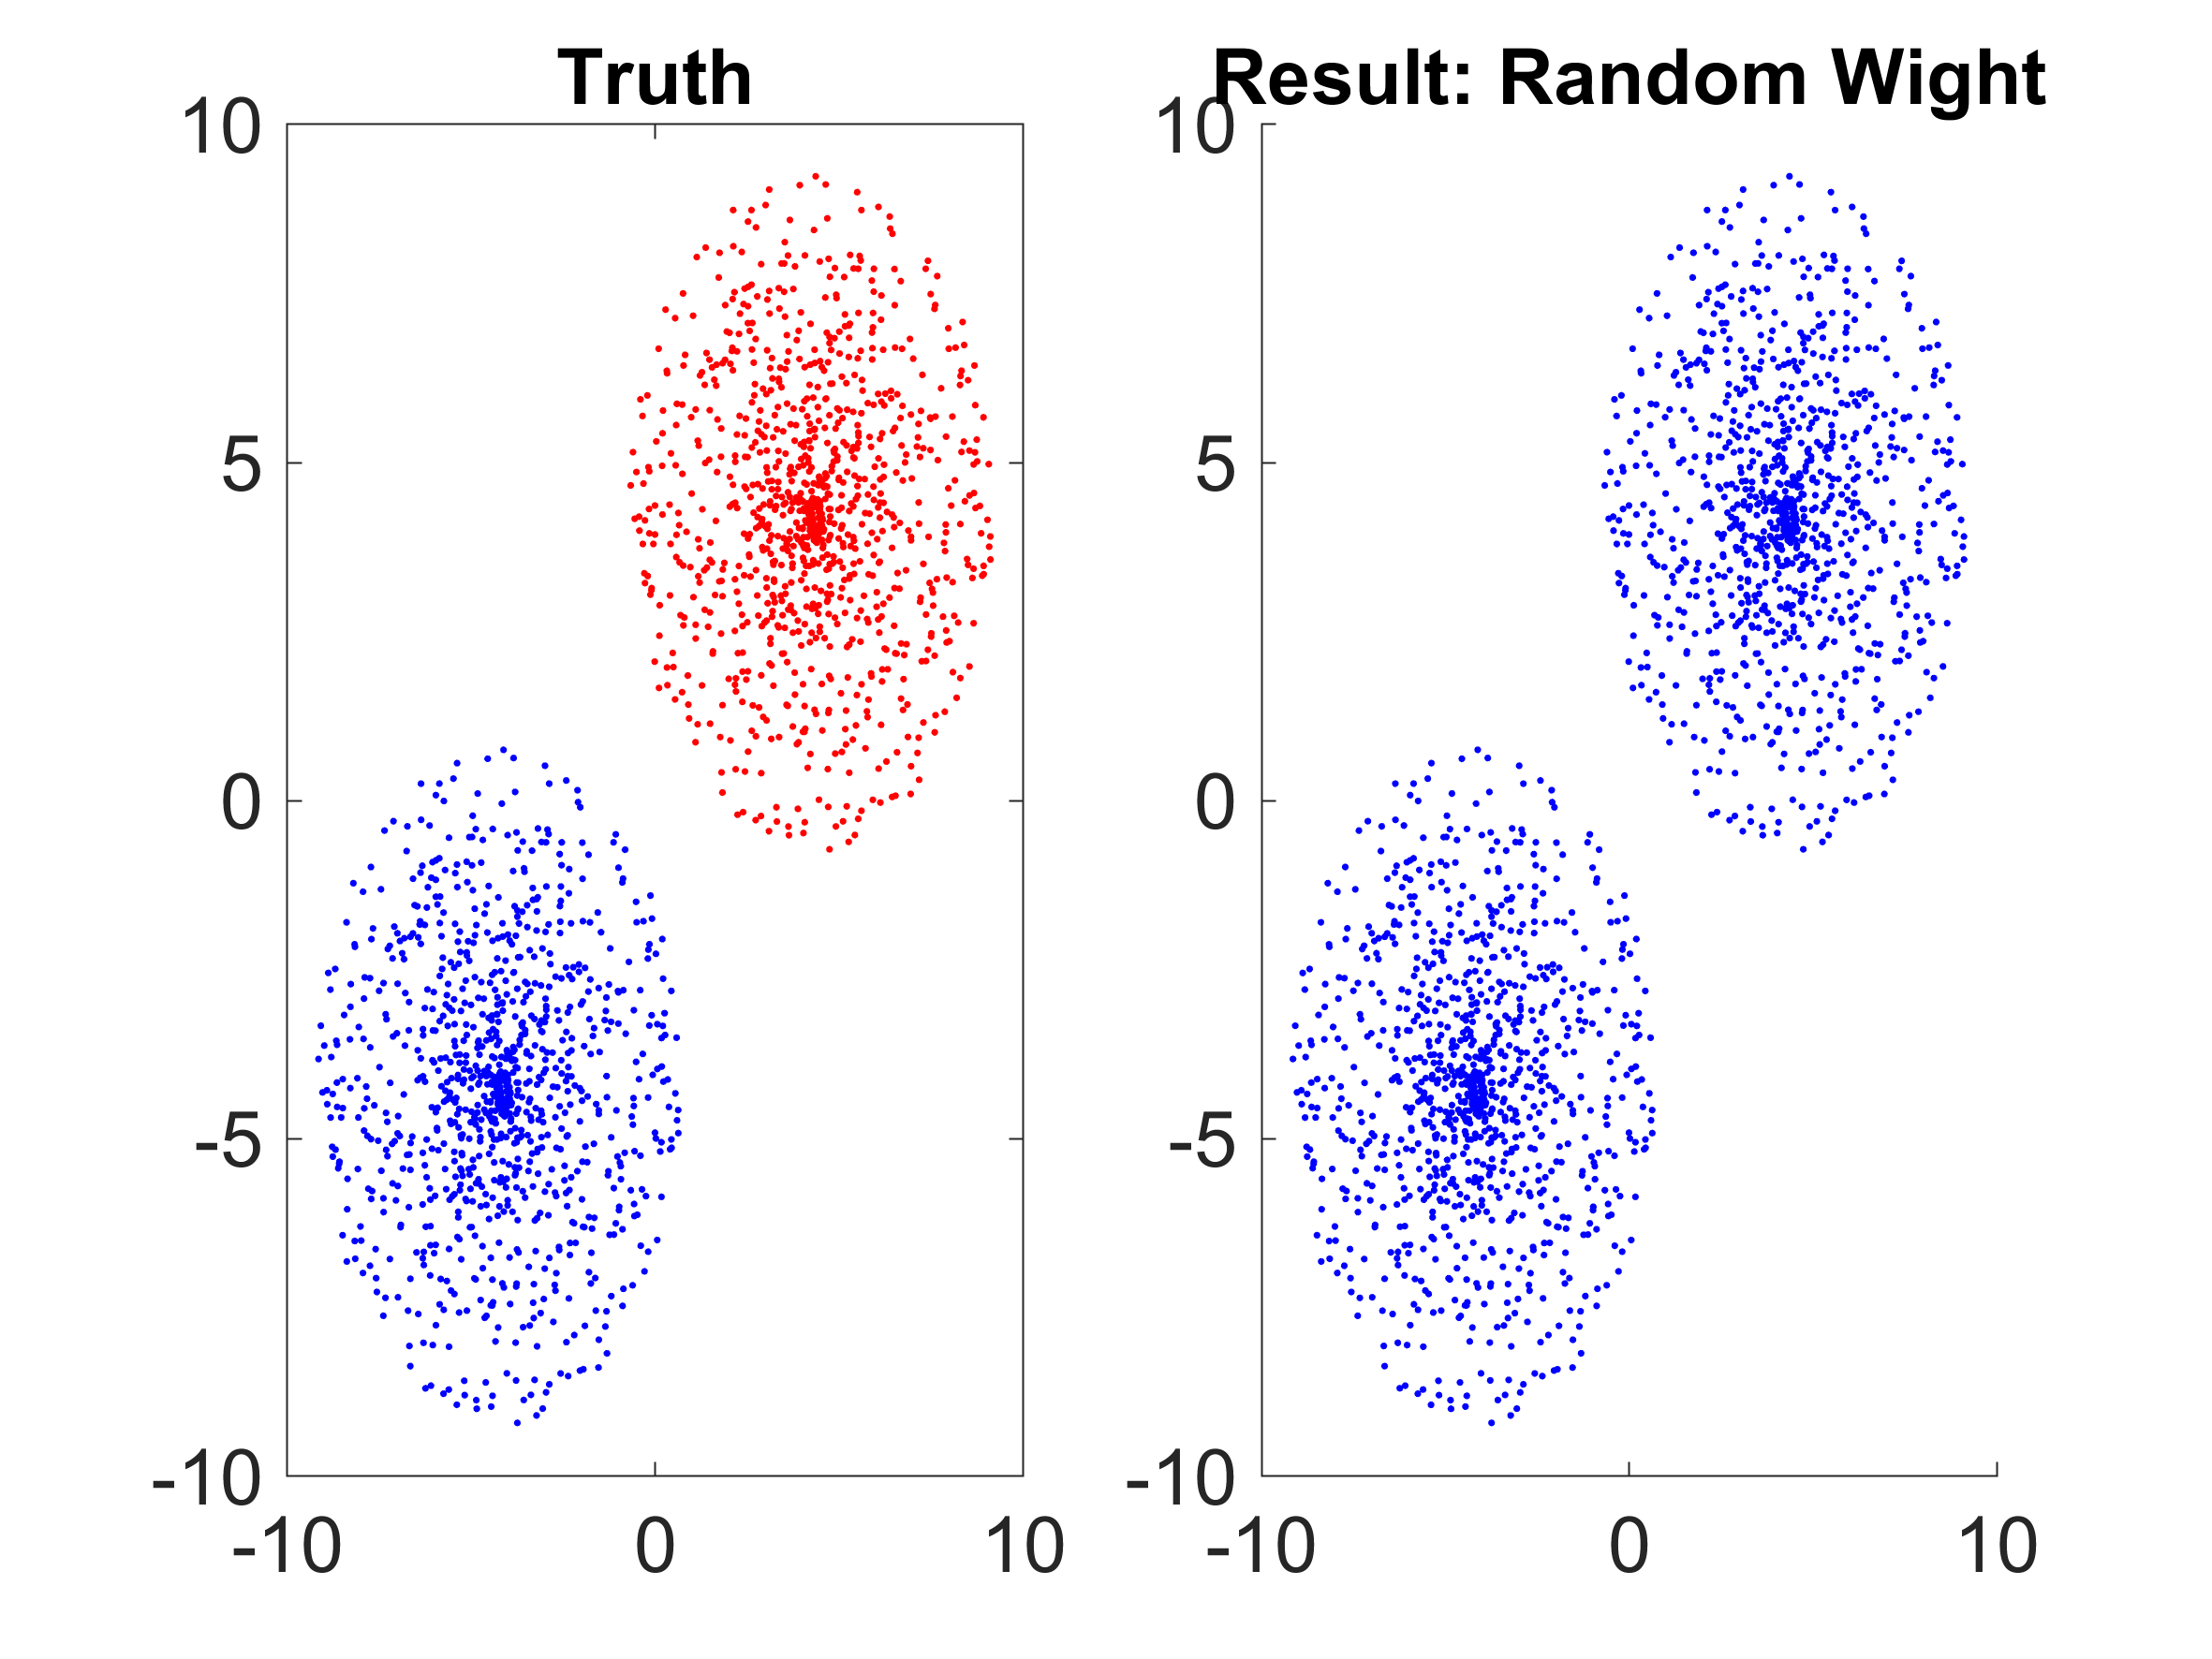
\includegraphics[width=0.45\textwidth]{./figures/ex2_1.png}
	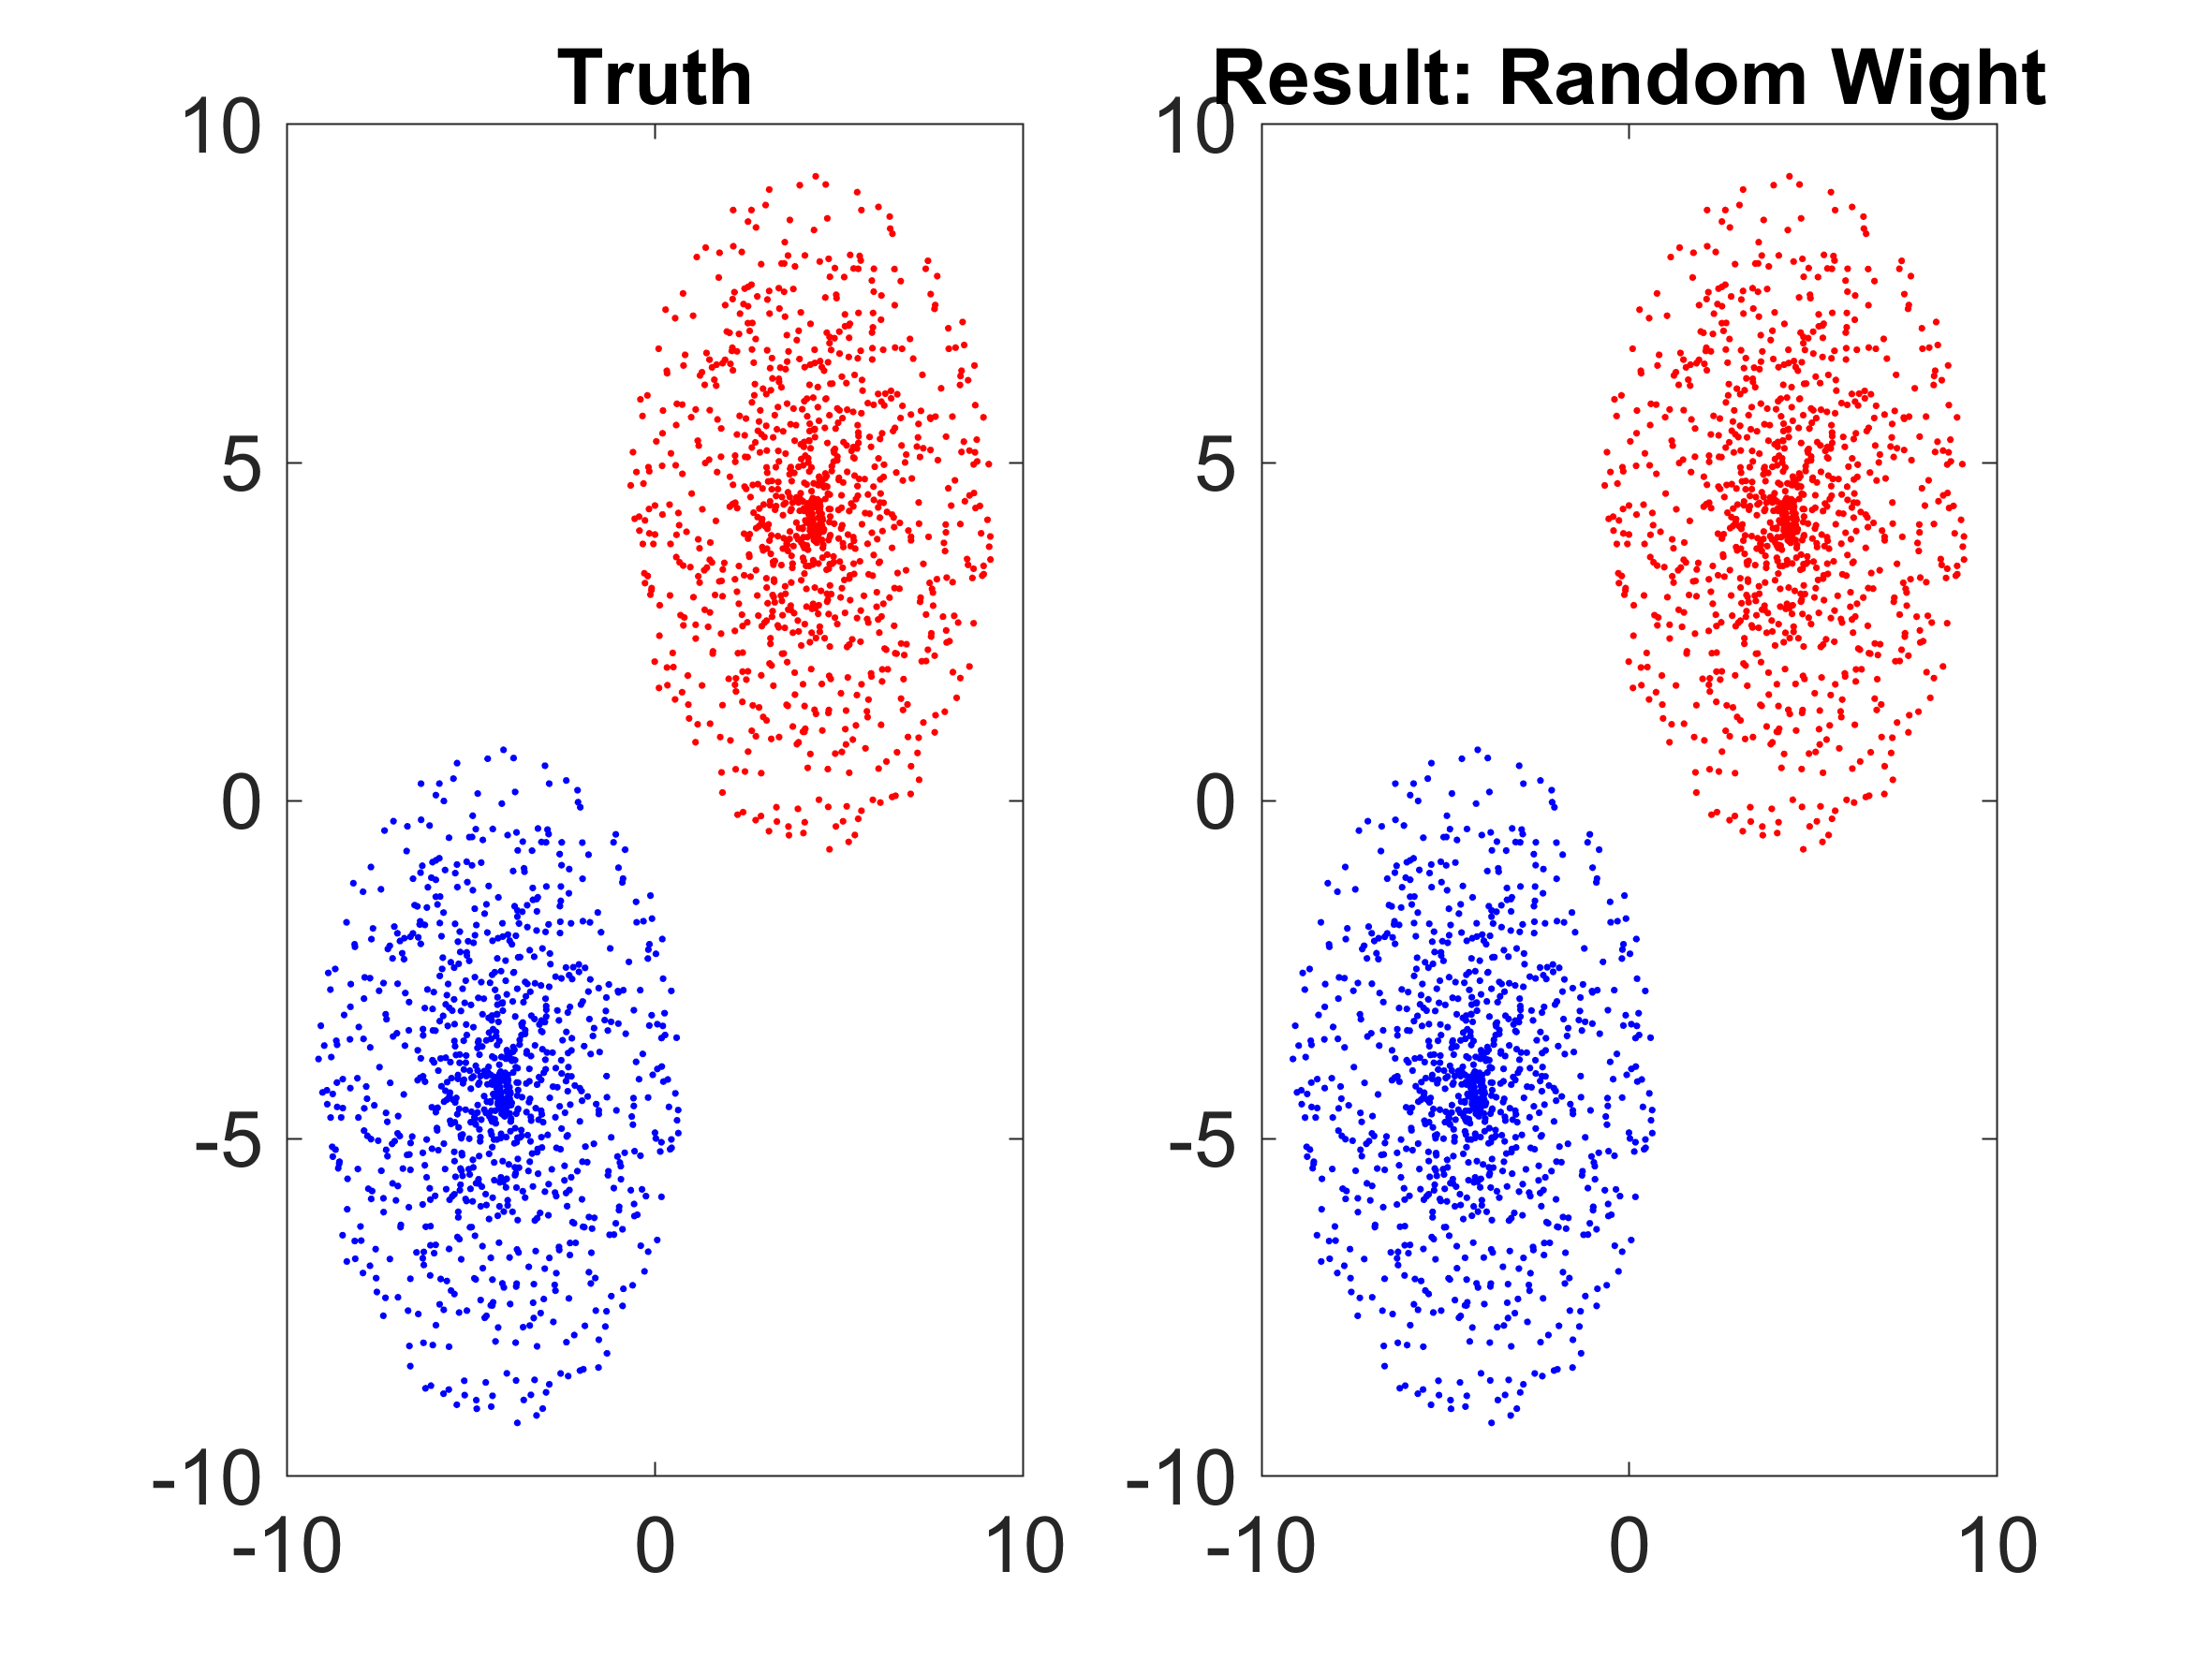
\includegraphics[width=0.45\textwidth]{./figures/ex2_2.png}
	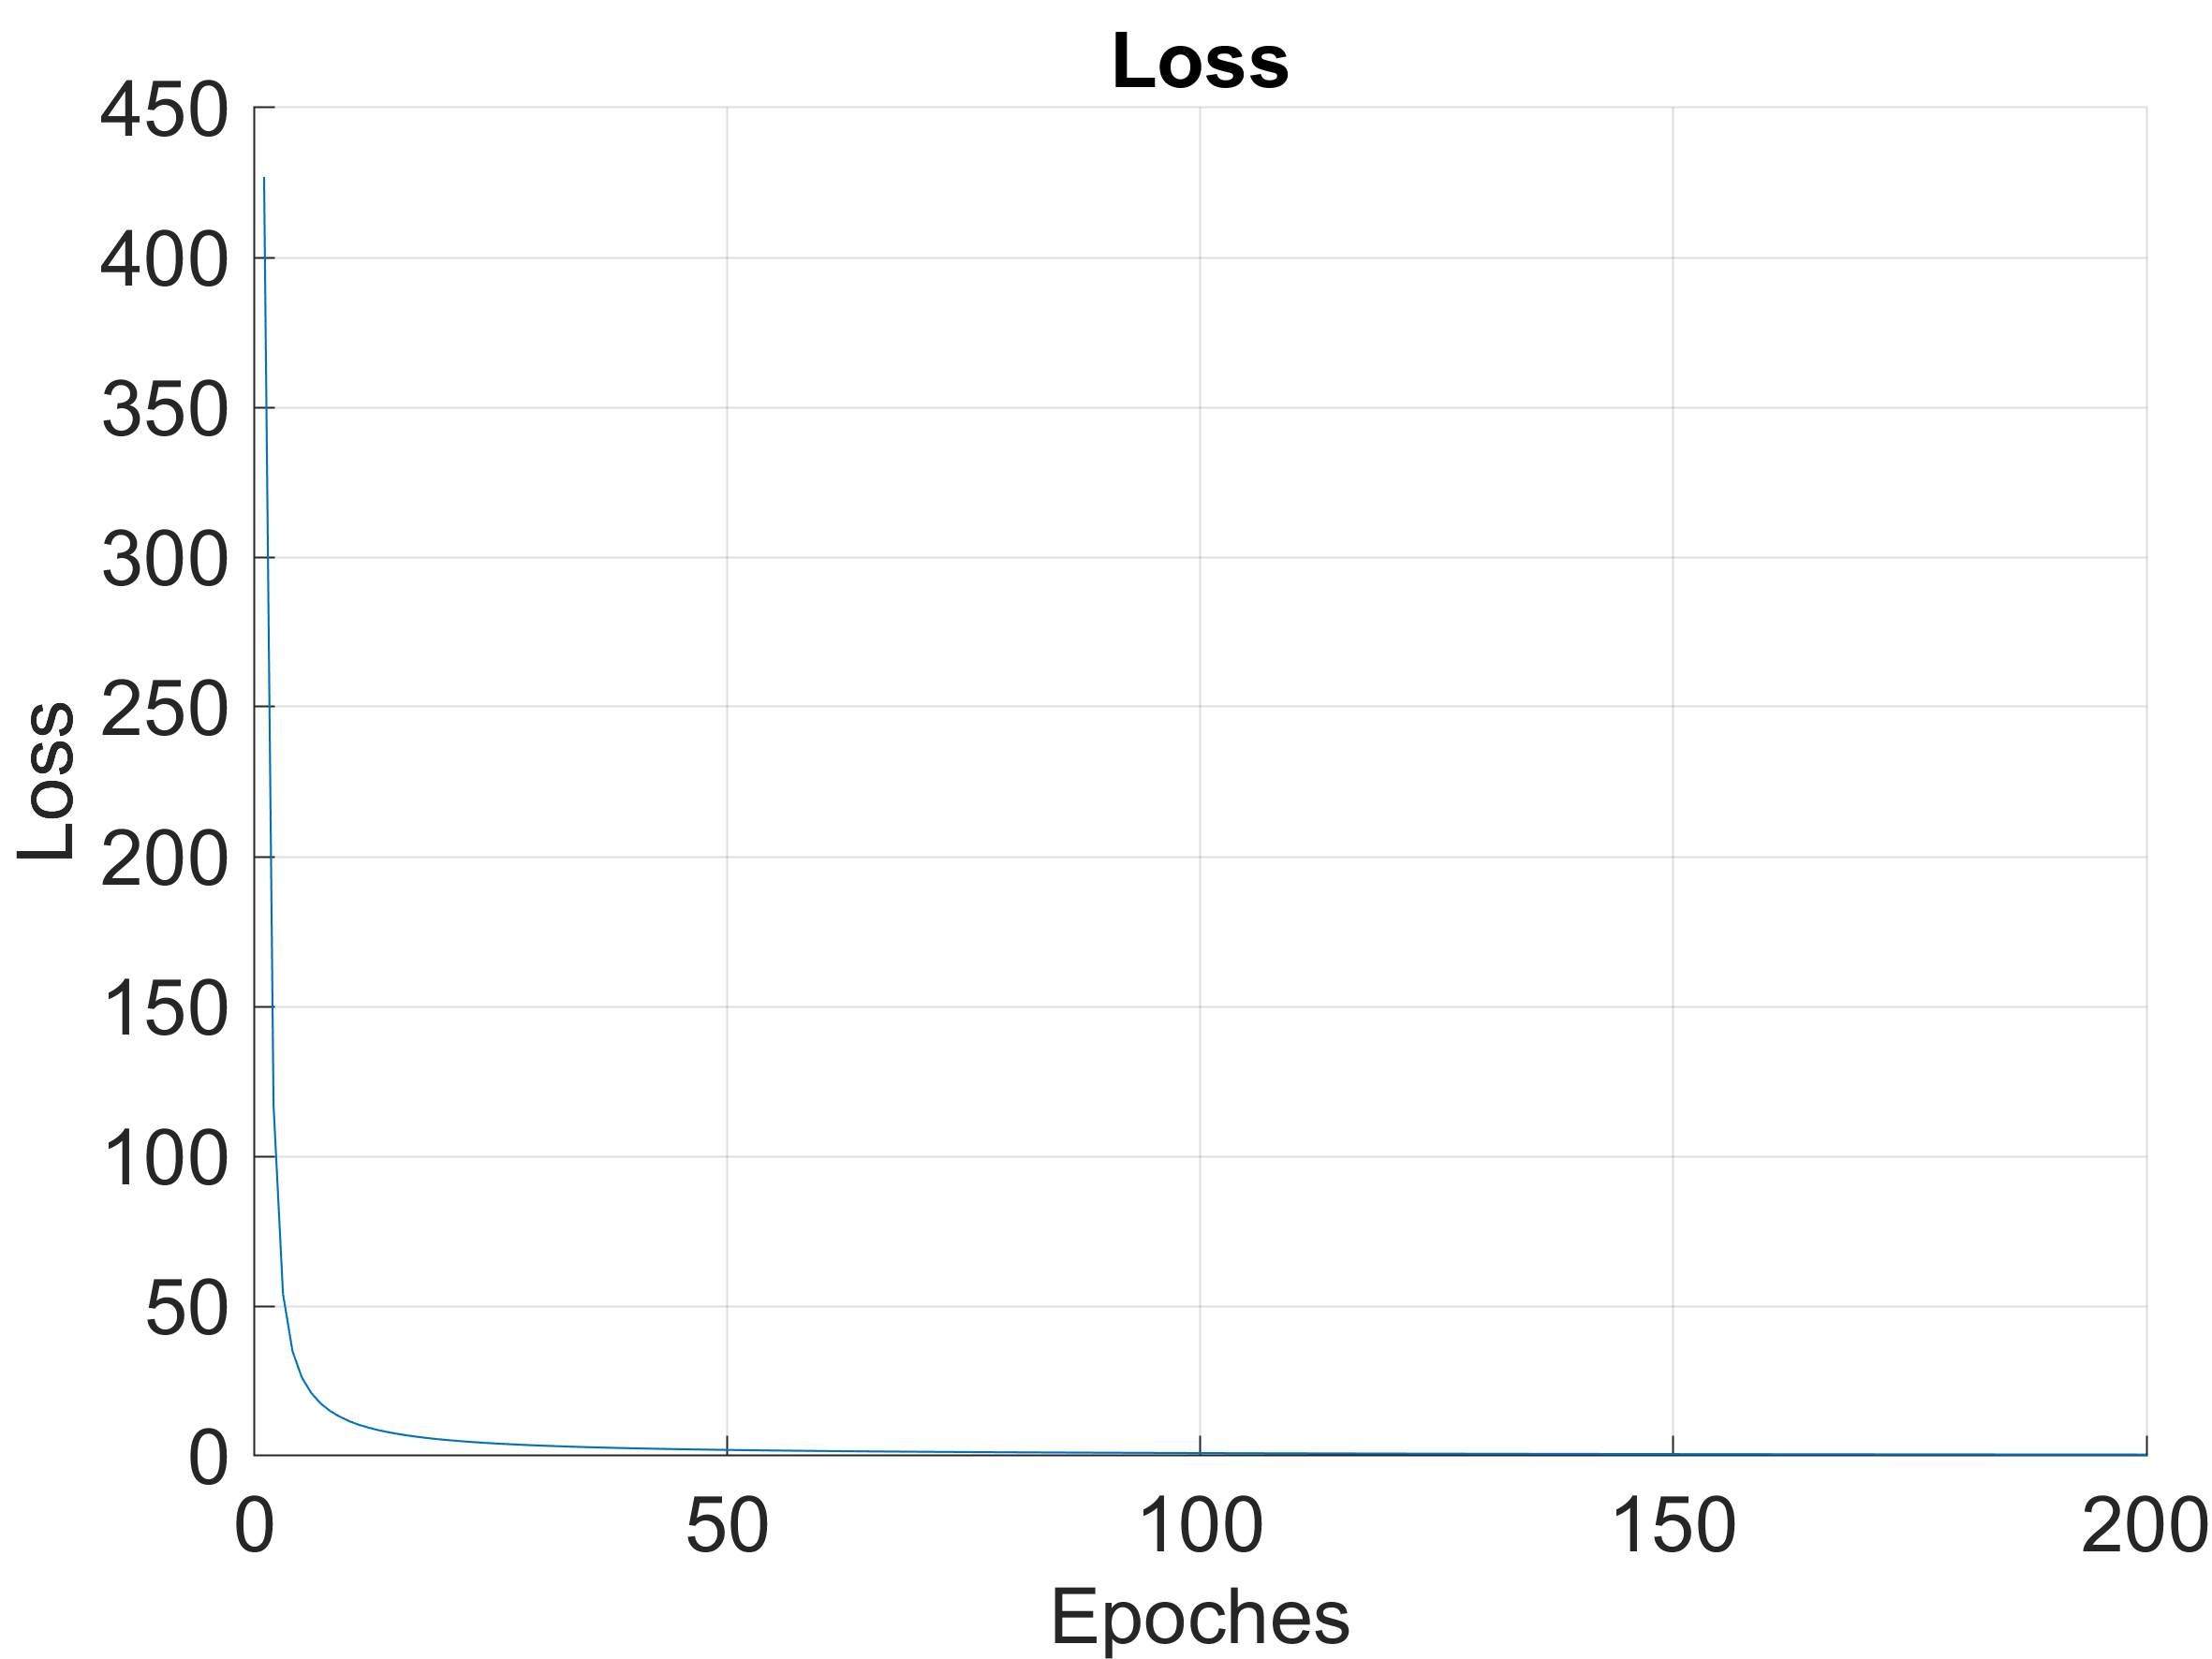
\includegraphics[width=0.45\textwidth]{./figures/ex2_3.png}
	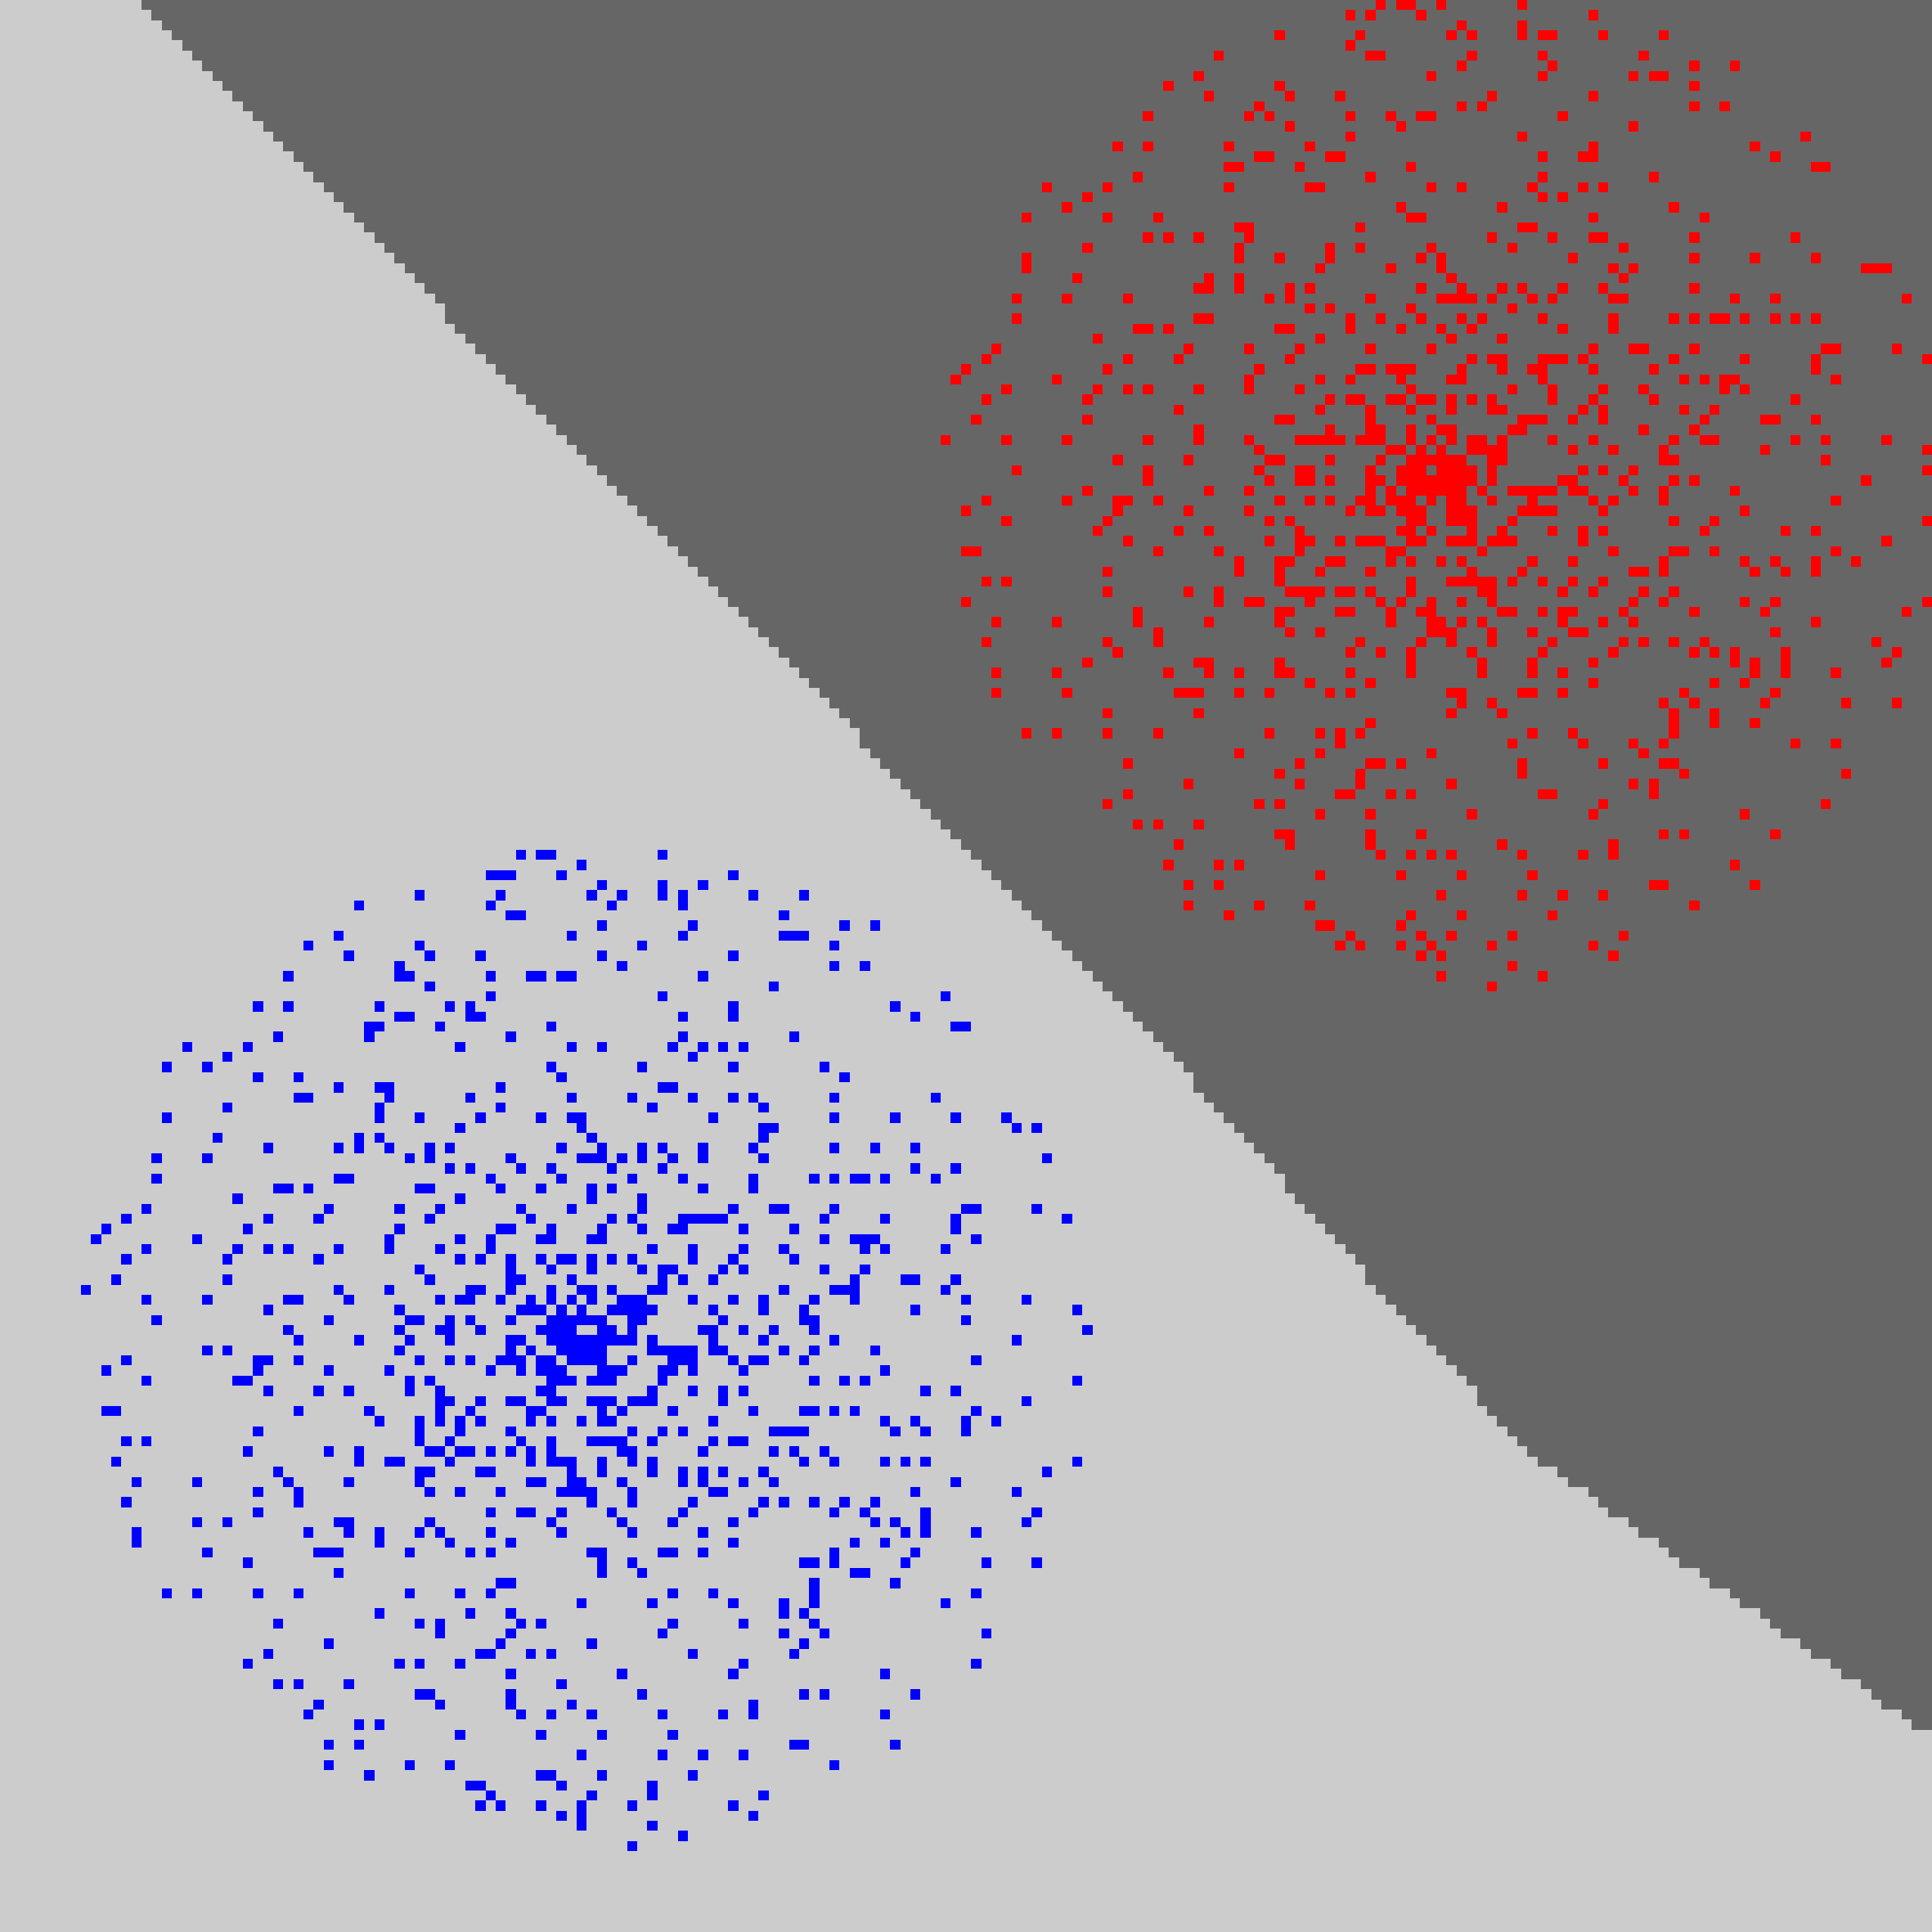
\includegraphics[width=0.45\textwidth]{./figures/ex2_4.png}
    \caption{$3$ layers neural network: 2x10x10x2.}
\end{figure*}

%	\begin{figure}[htbp]
%	\centering
%	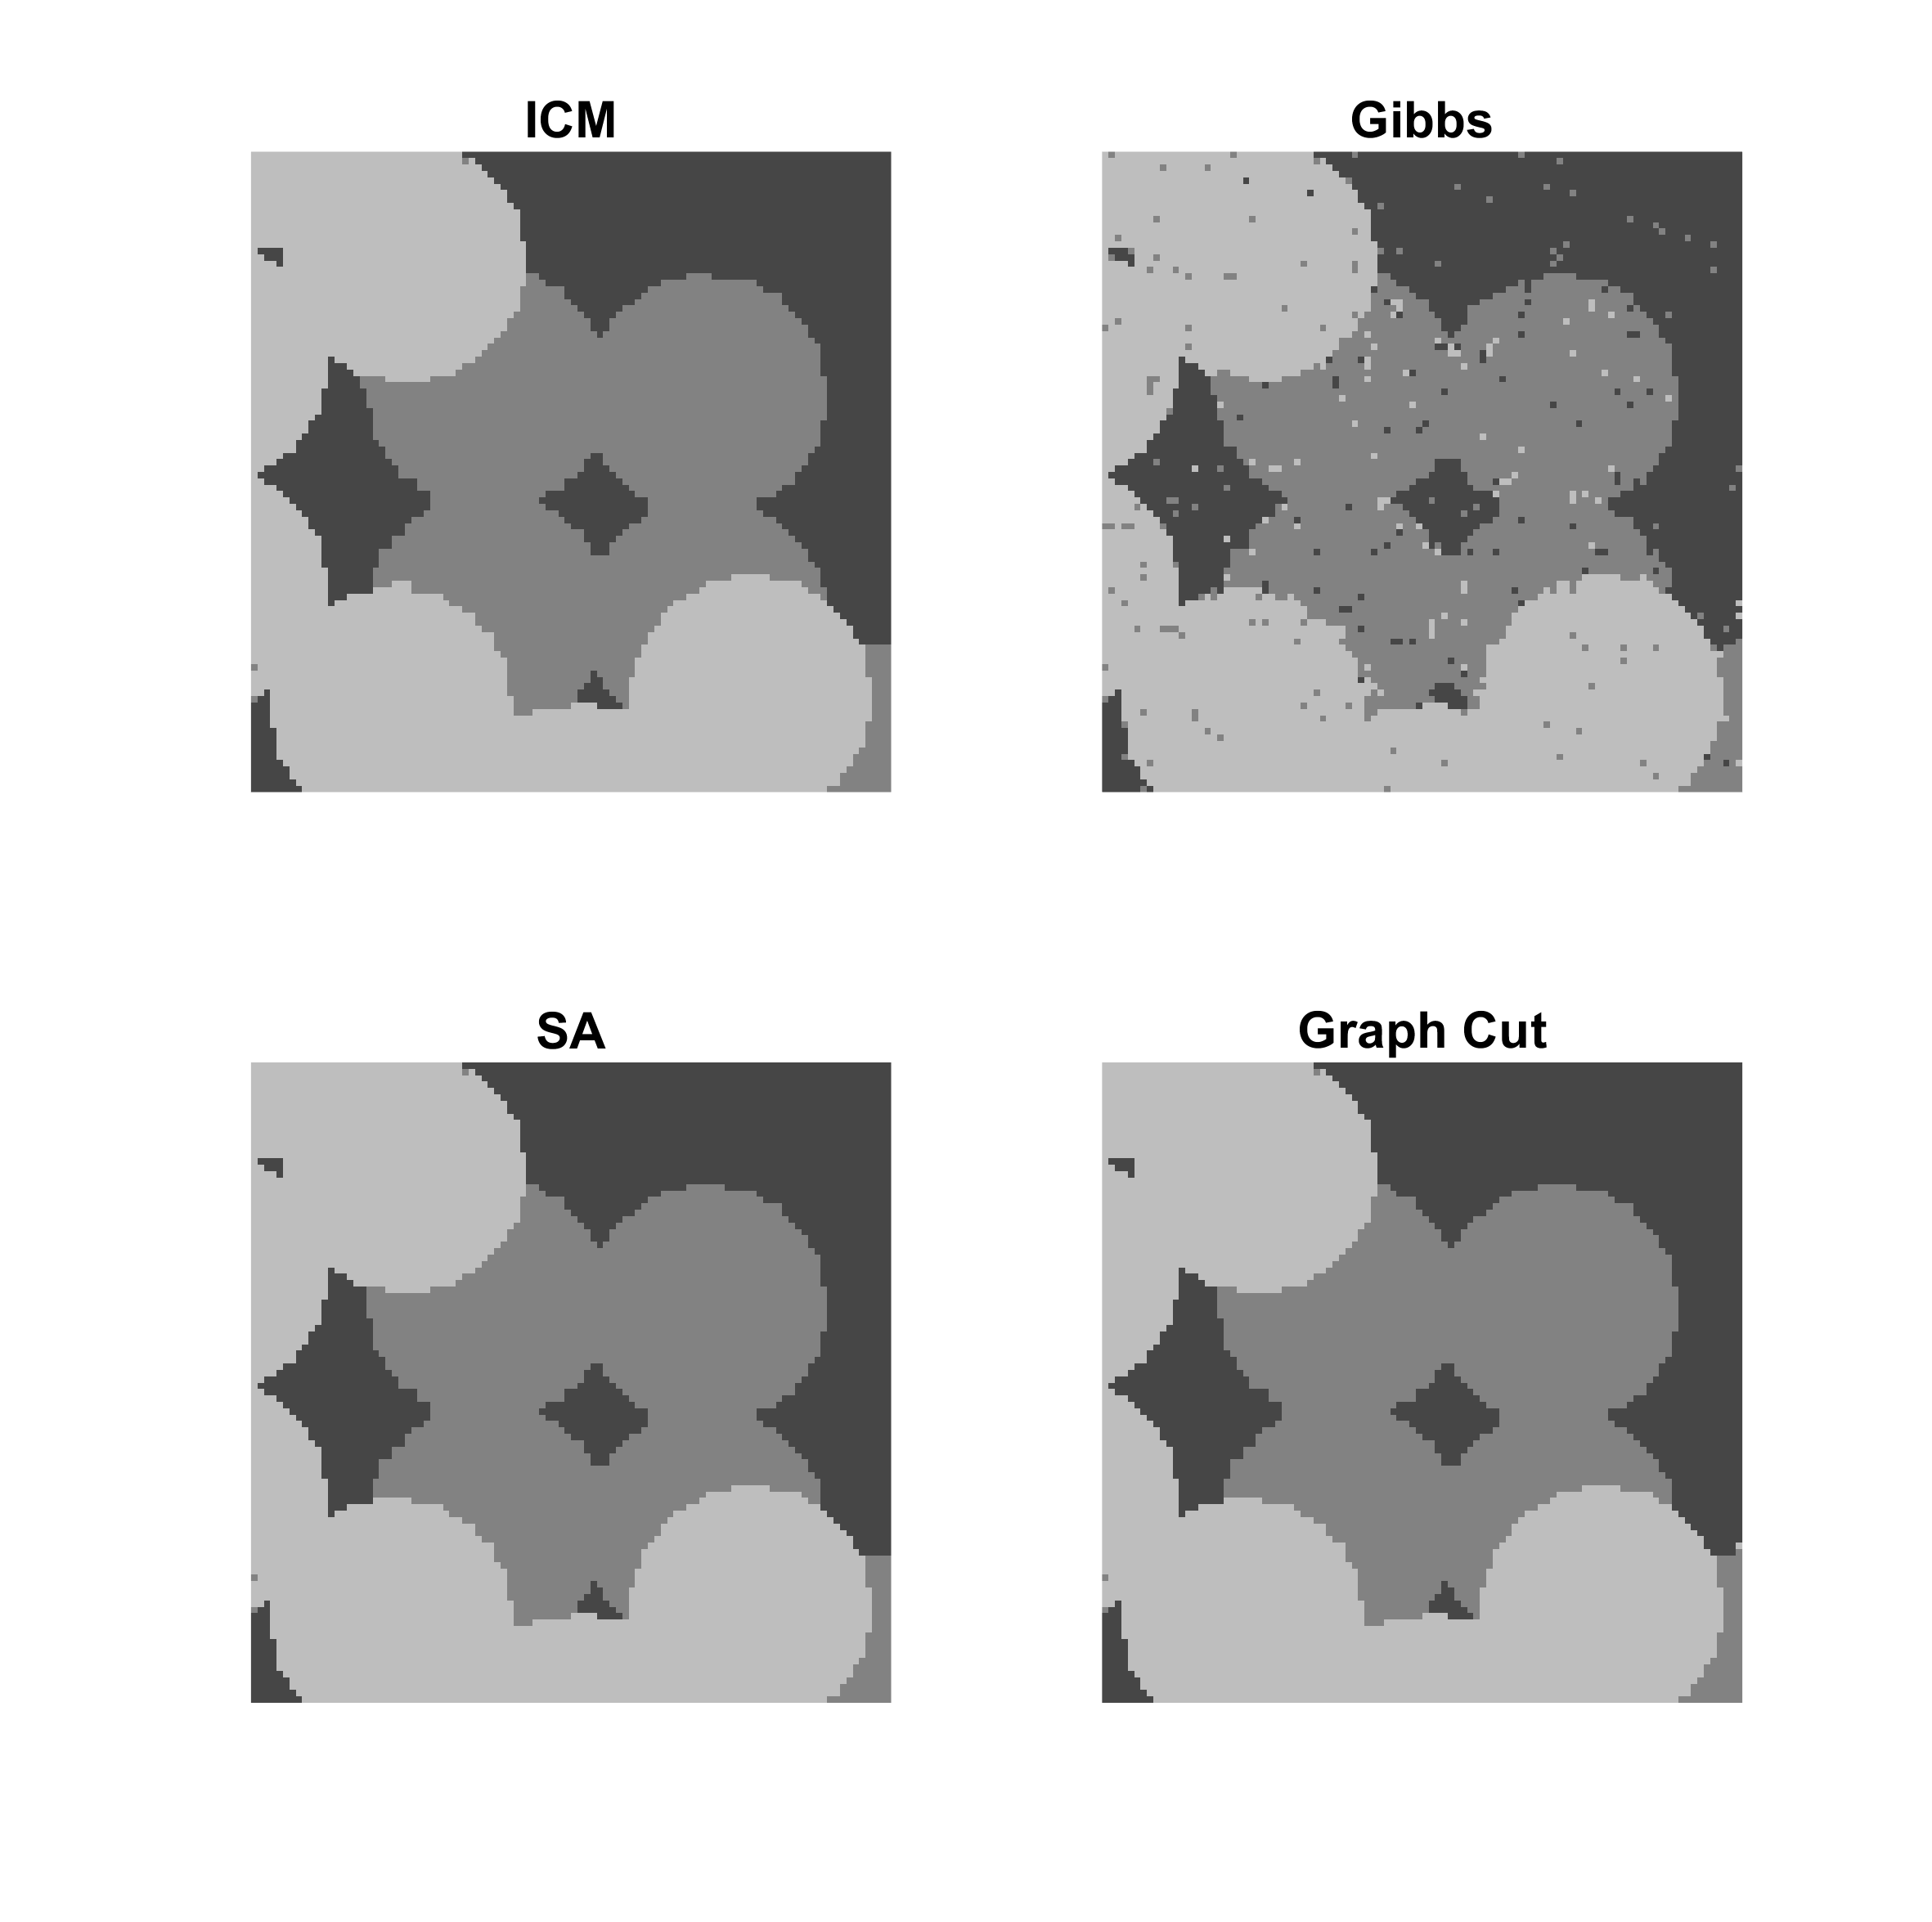
\includegraphics[width=0.6\textwidth]{./figures/cmp1.png}
%	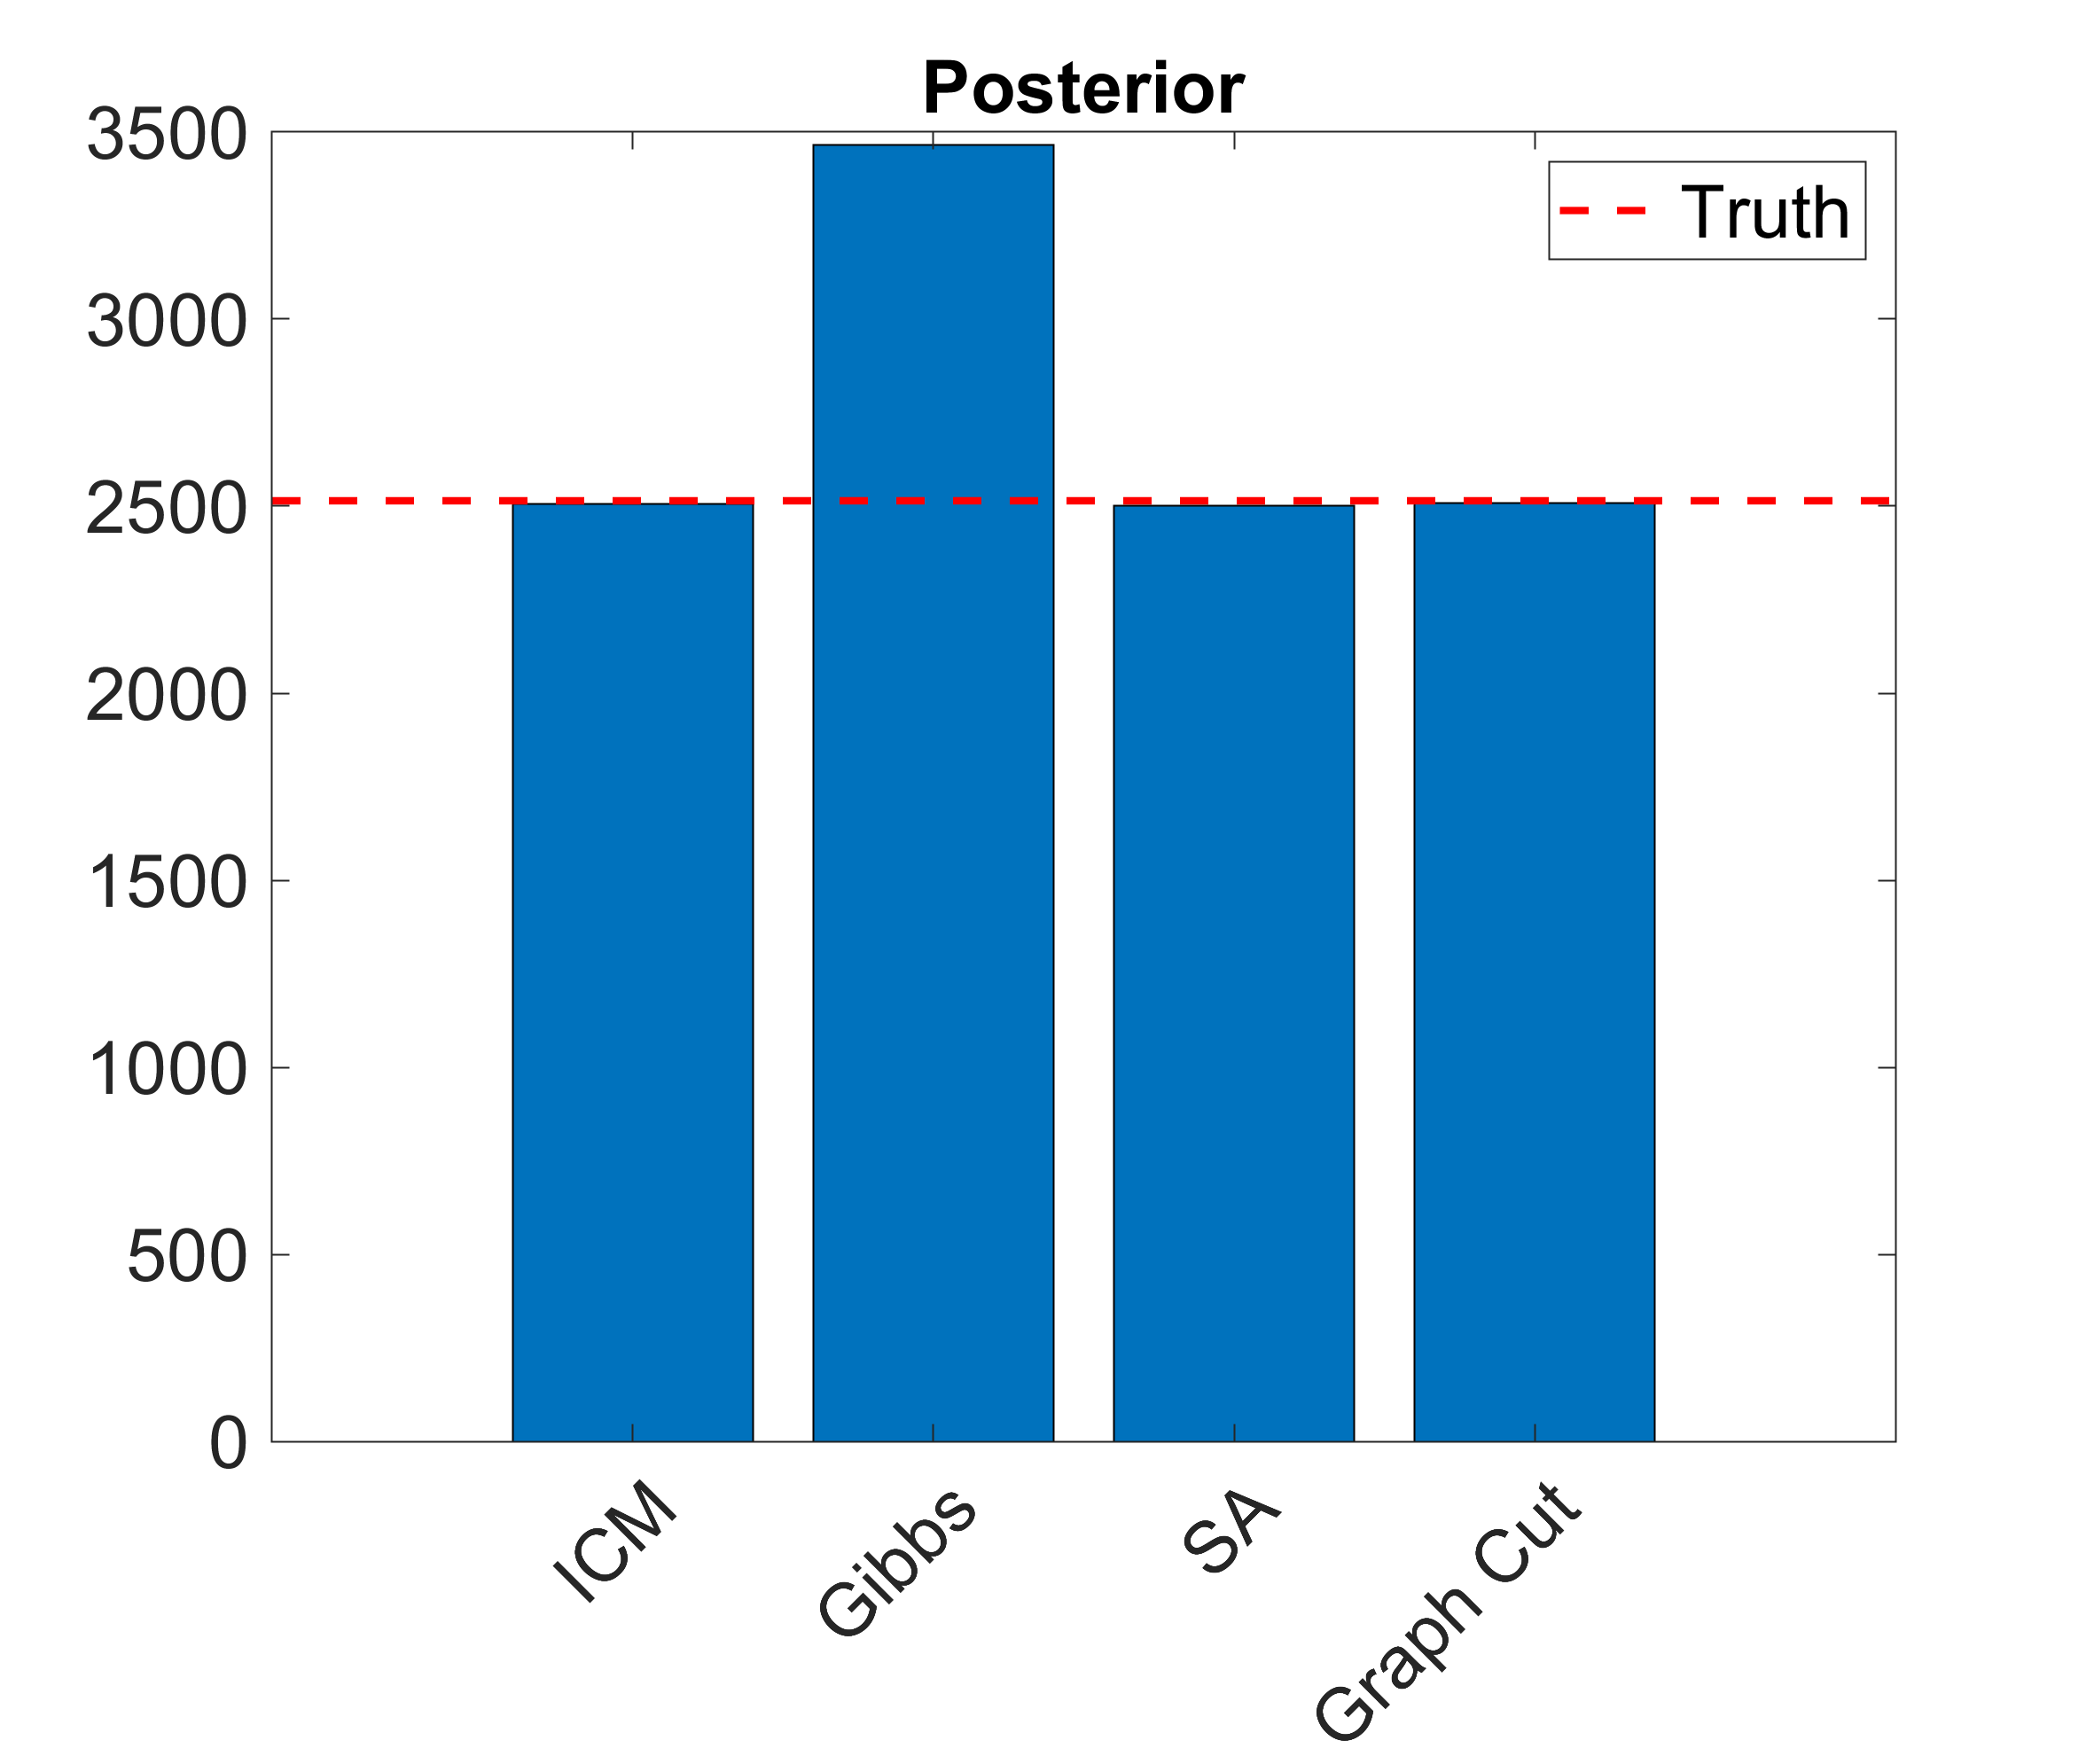
\includegraphics[width=0.38\textwidth]{./figures/cmp2.png}
%    \caption{Comparison of using MRF with different optimization approaches. Visually speaking, ICM, Simulated Annealing, and Graph Cut give better performance than the Gibbs Sampling method. The right image shows the cost of the four optimization approaches. It is clear that ICM, SA, and Graph Cut all achieves the ground truth. However, local optimization method like ICM cannot always guarantee to achieve the global minimum. SA, however, is probabilistic optimum. So with the iteration increasing, its probability of achieving global optimum will increase up to 1. Graph cut is a globally optimal method for binary label segmentation.}
%\end{figure}
%
%	\begin{figure}[htbp]
%	\centering
%	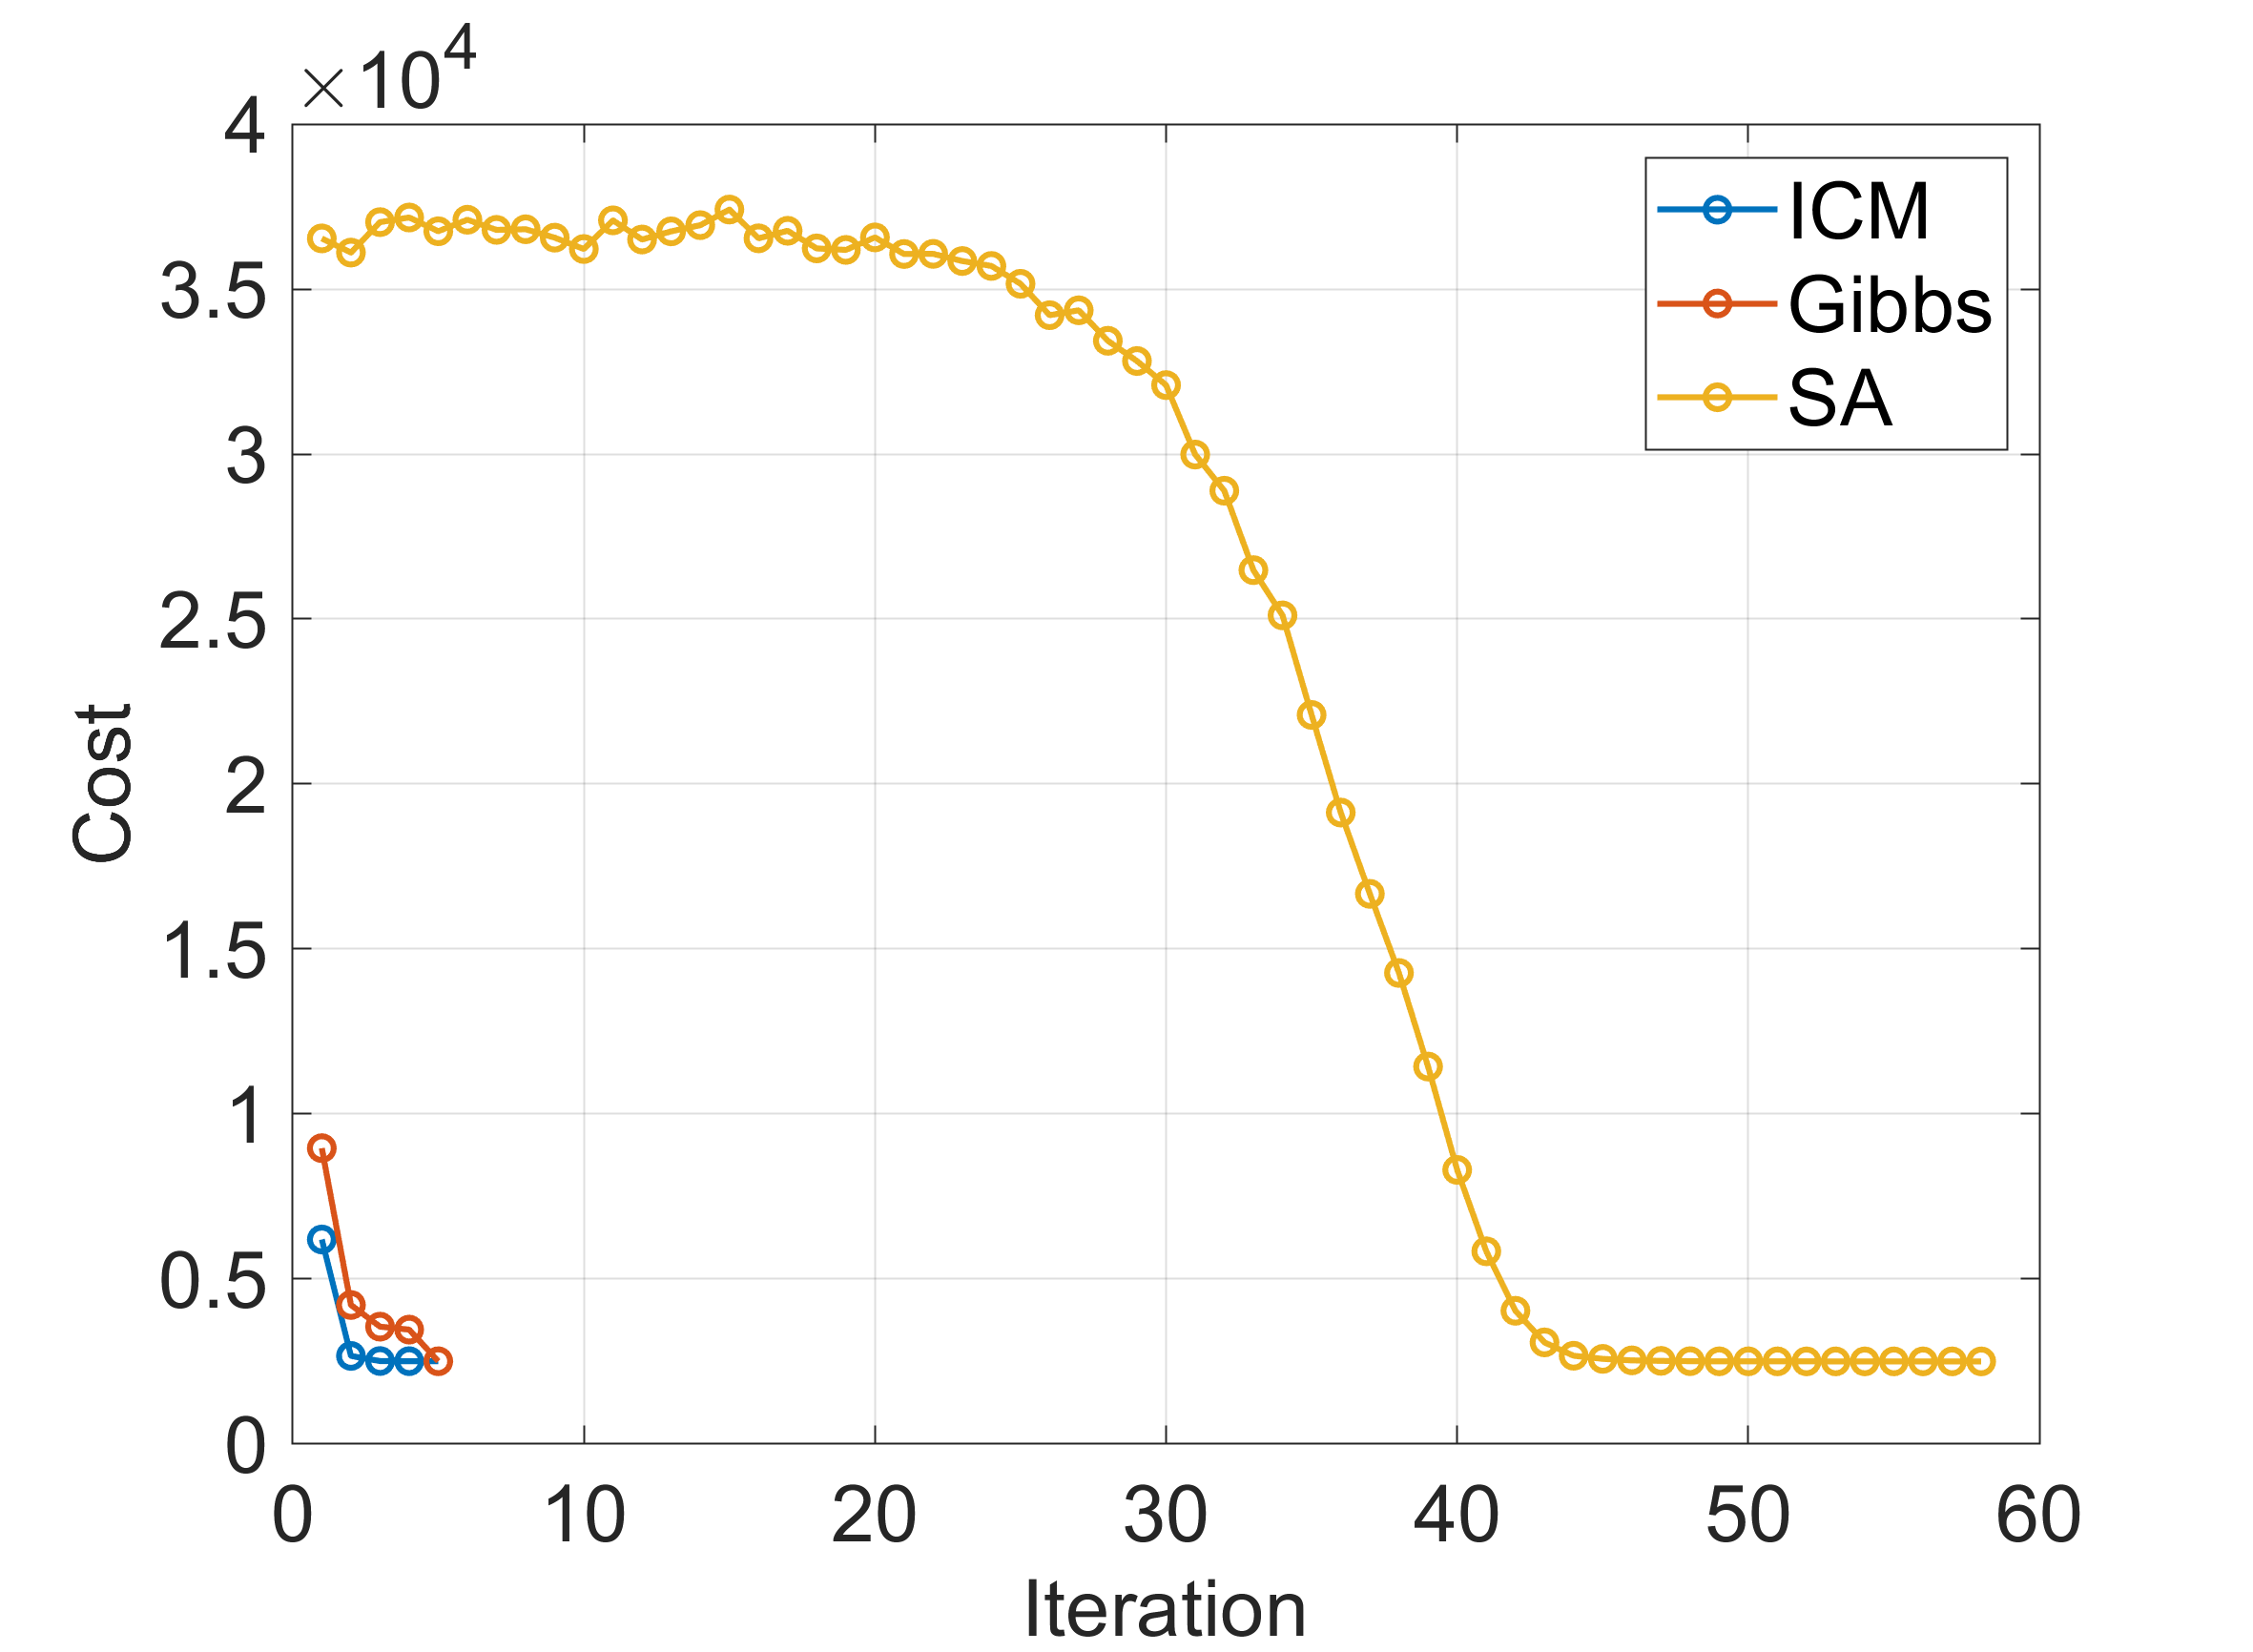
\includegraphics[width=0.5\textwidth]{./figures/cmp.png}
%    \caption{Iteration comparison: SA will use more iteration to converge because it needs the temperature to be cooled down. Faster convergence can be achieved by make temperature cool down faster at the expense of increasing the possibility of being trapped in a local minimum. ICM and Gibbs sampling methods can converge rapidly compared with SA.}
%\end{figure}
%
%	\begin{figure}[htbp]
%	\centering
%	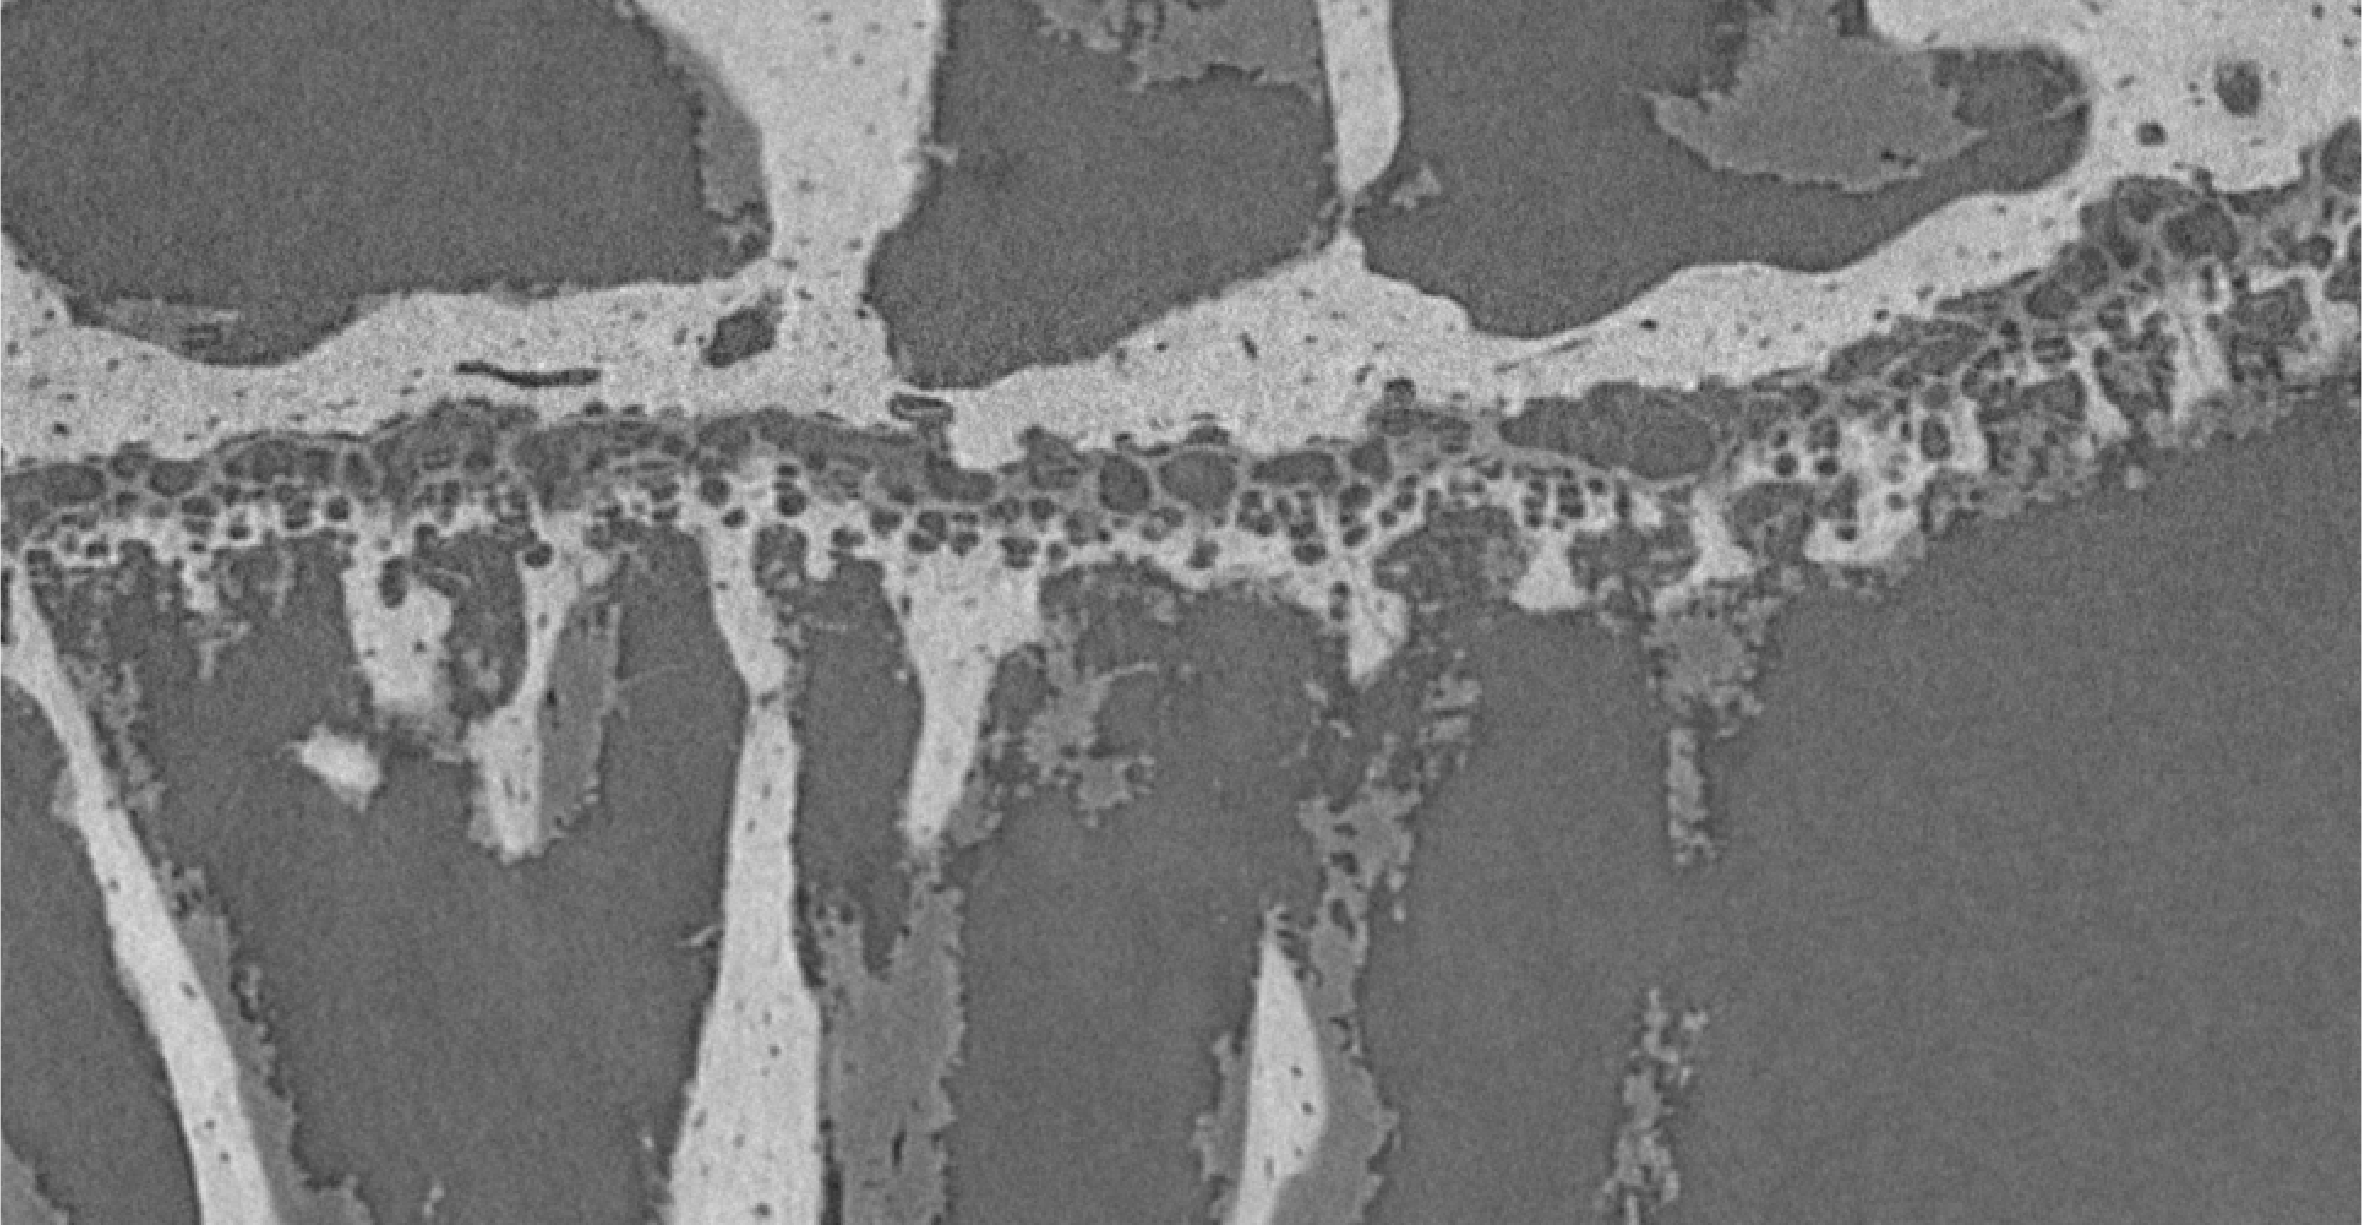
\includegraphics[width=0.5\textwidth]{./figures/assign2_raw.png}
%	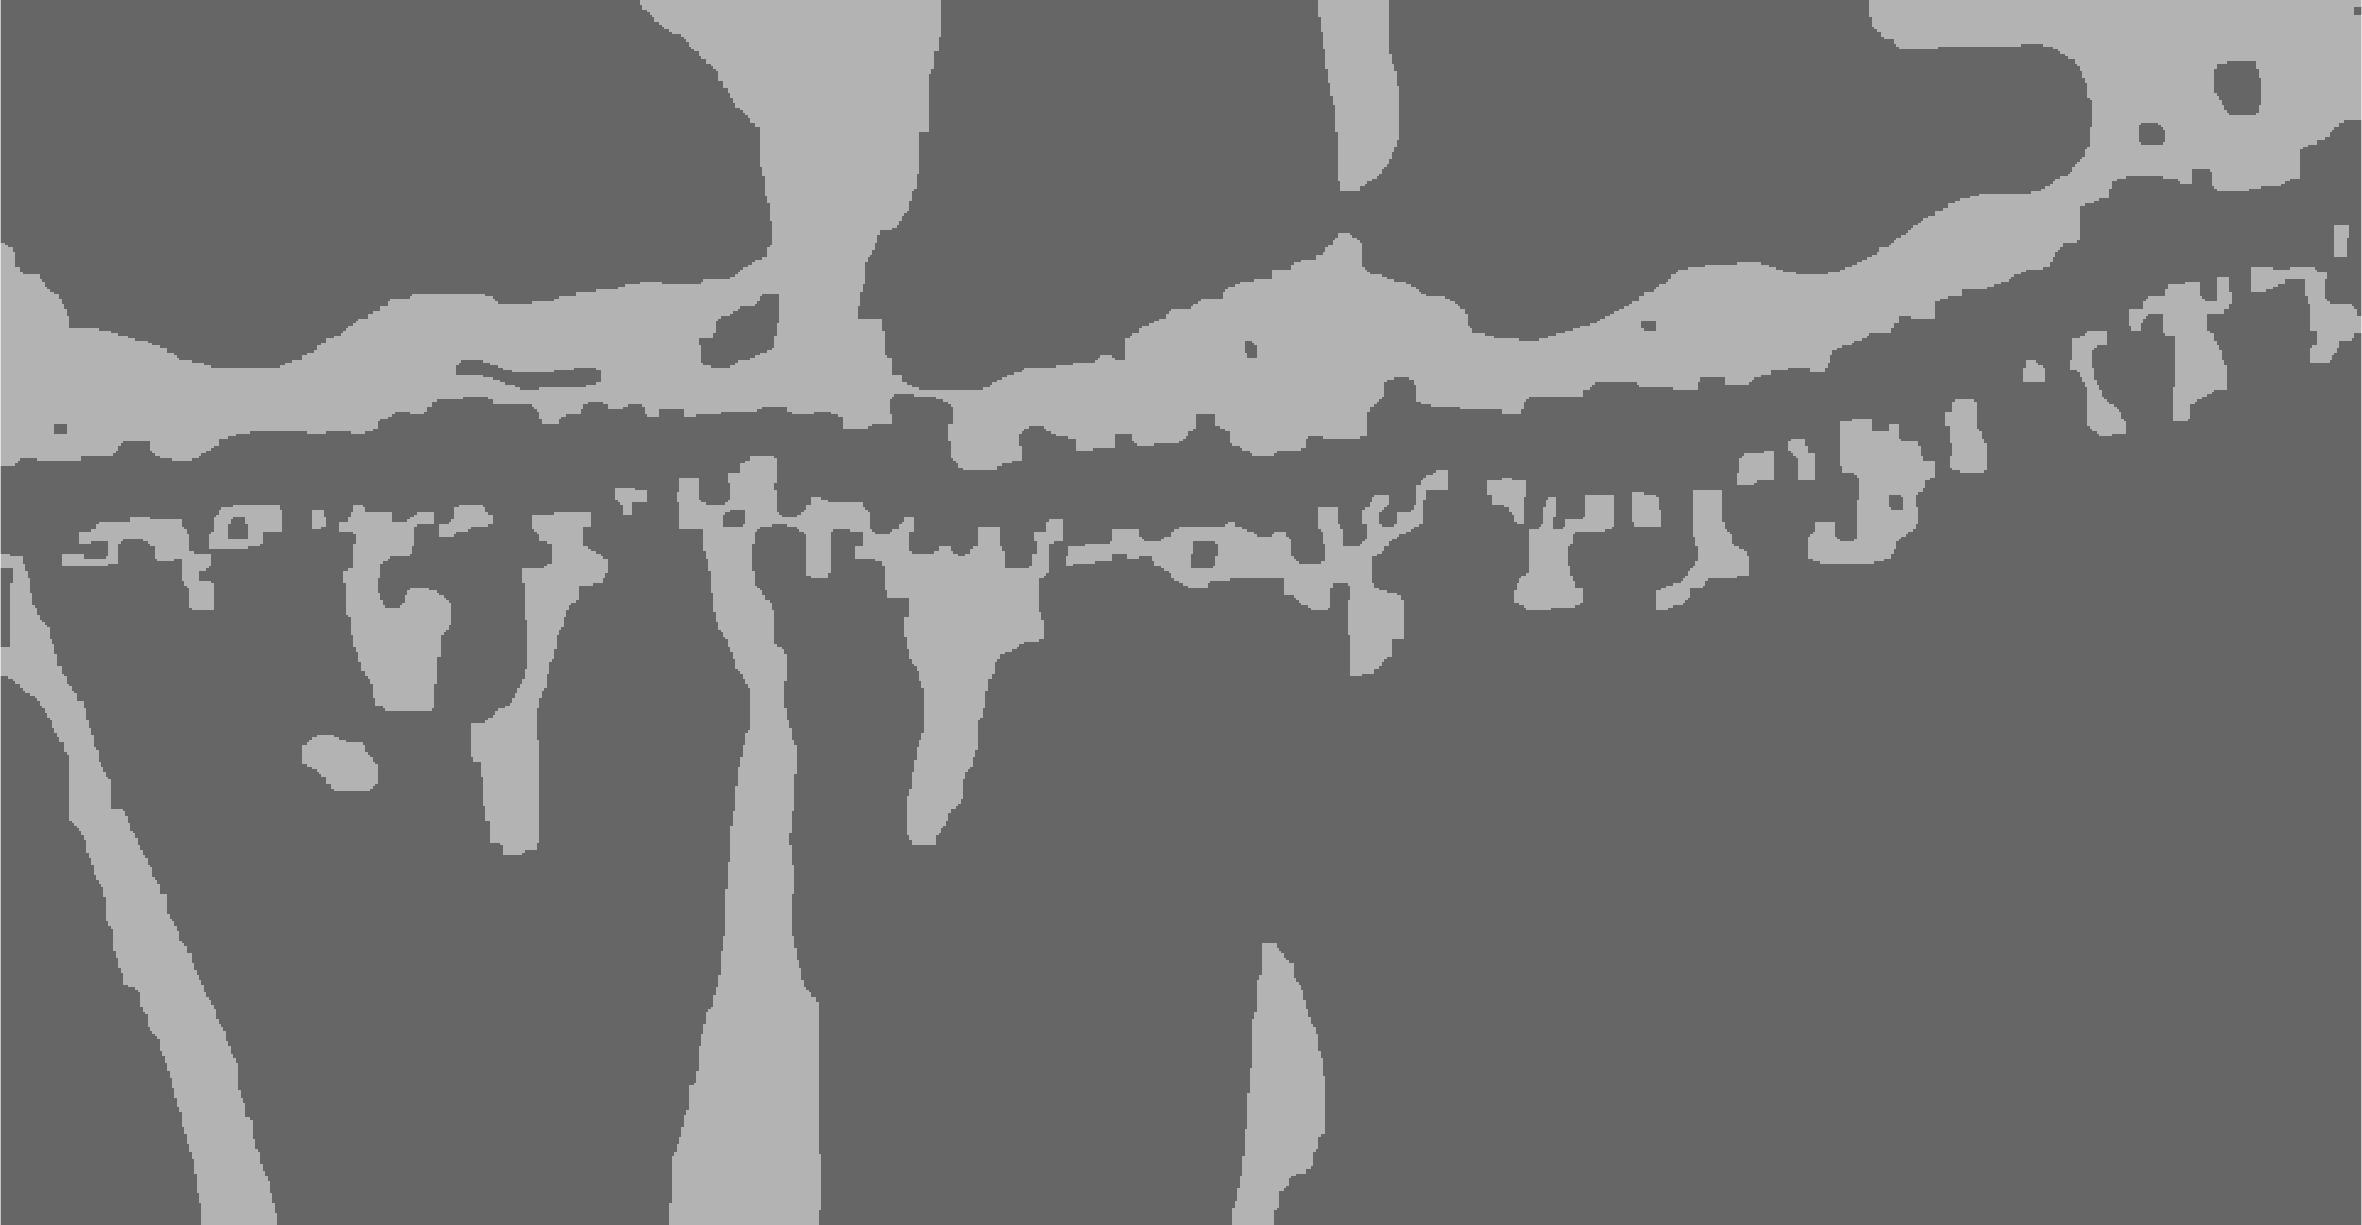
\includegraphics[width=0.5\textwidth]{./figures/assign2_seg.png}
%	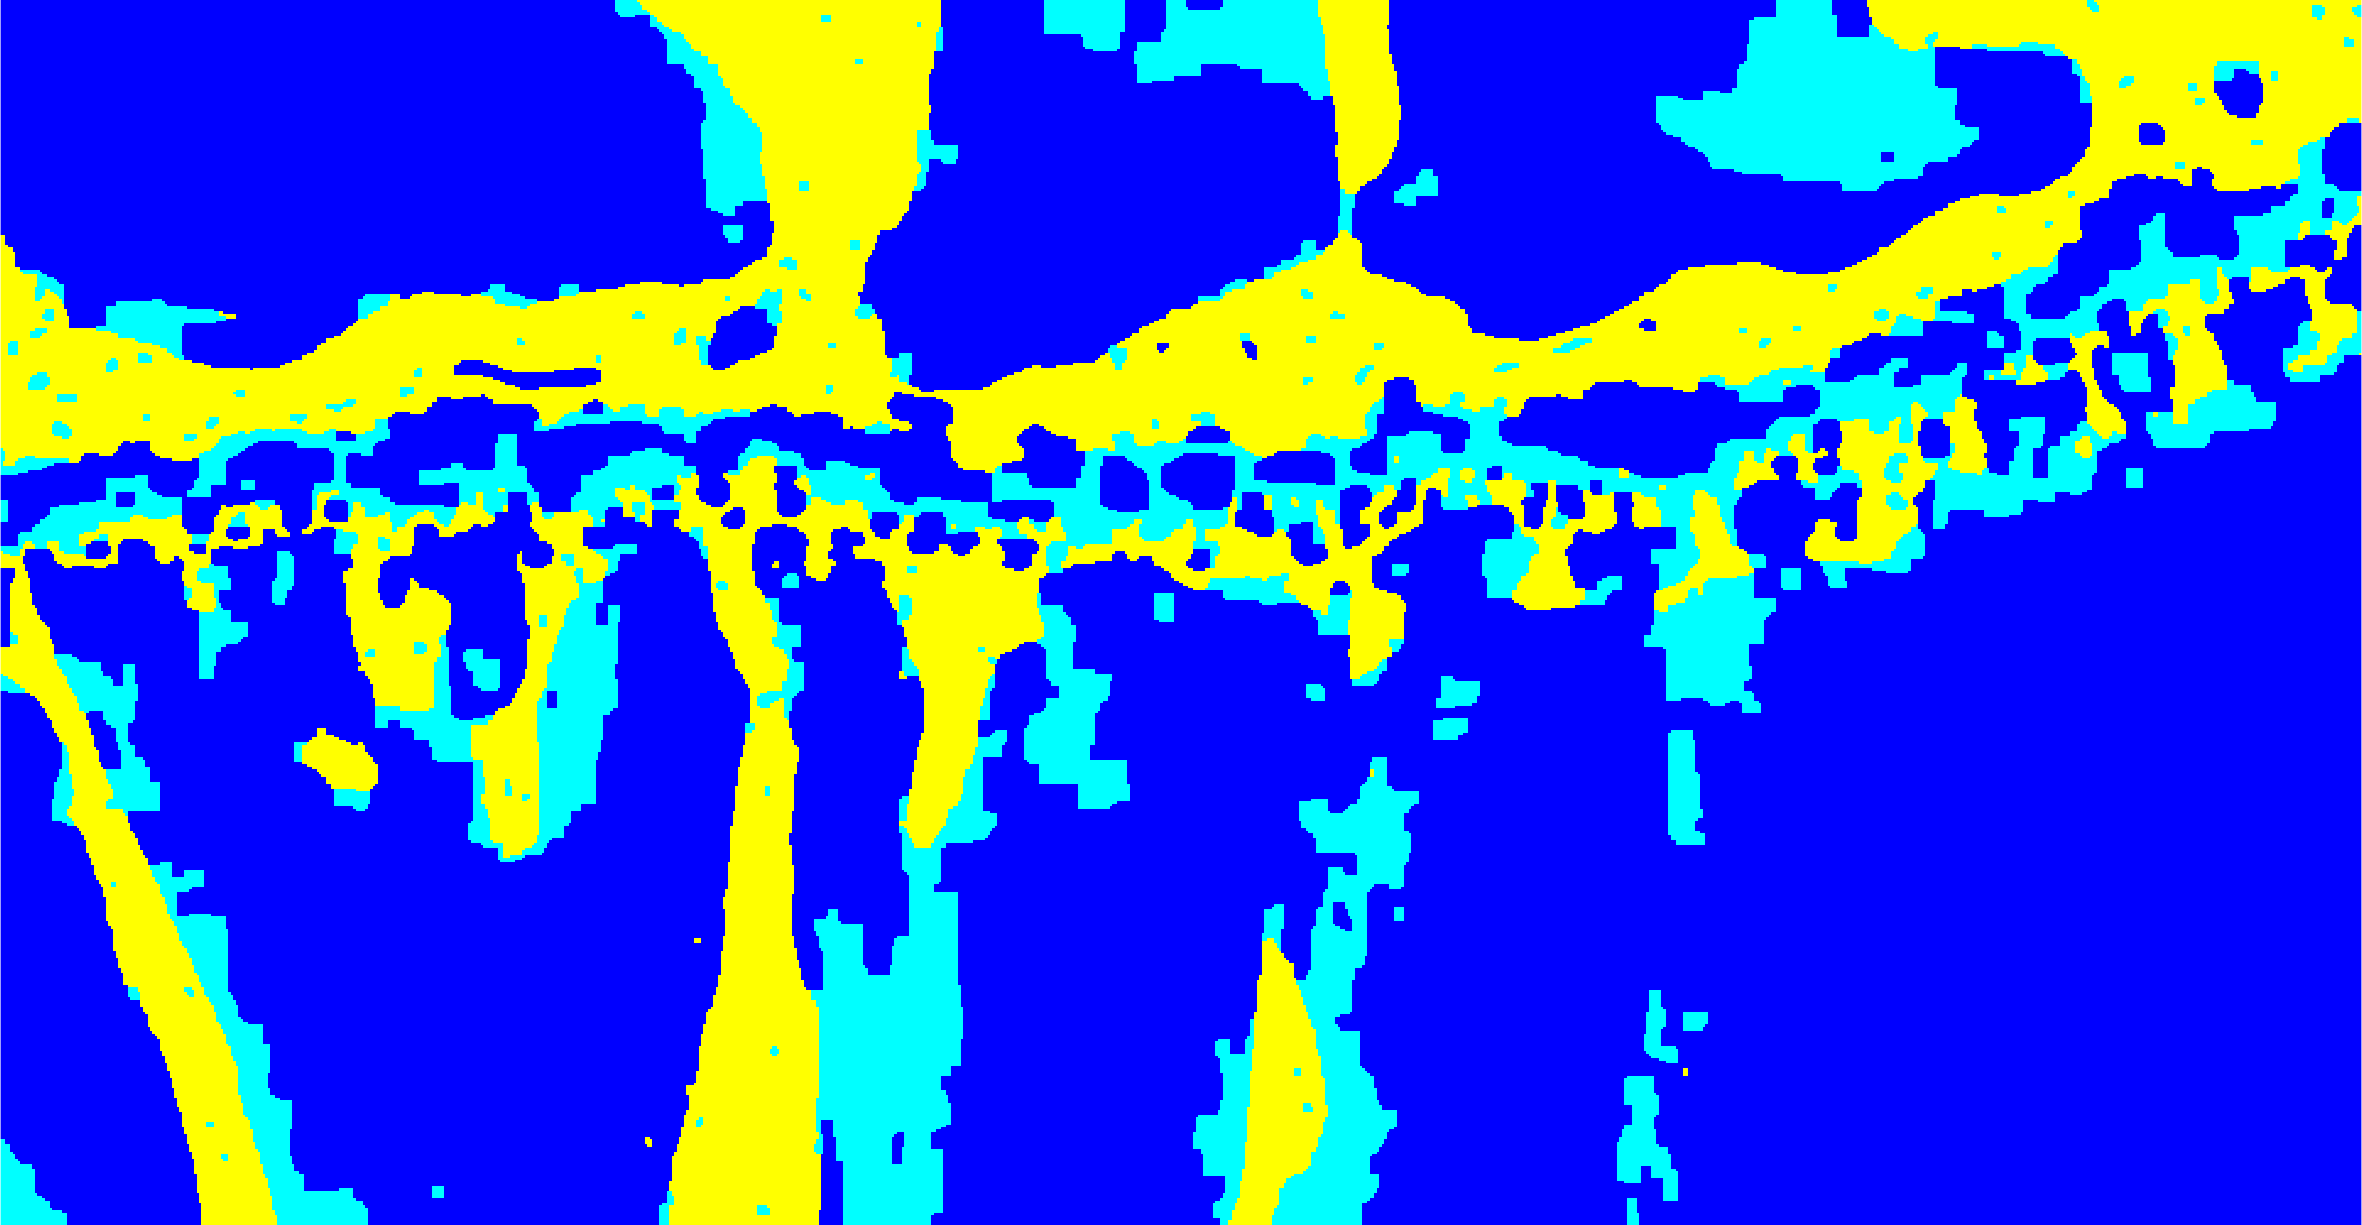
\includegraphics[width=0.5\textwidth]{./figures/assign2_mseg.png}
%    \caption{Middle image shows the segmentation of bone (bright) and air (dark). The bottom image shows the segmentation of bone (yellow), cartilage (light blue), and air (dark blue).}
%\end{figure}
%	\section{Deformable Models}
%	\begin{figure}[htbp]
%	\centering
%	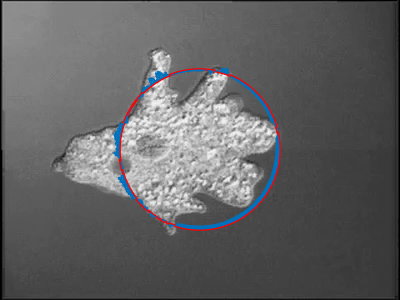
\includegraphics[width=0.45\textwidth]{./figures/defom1.png}
%	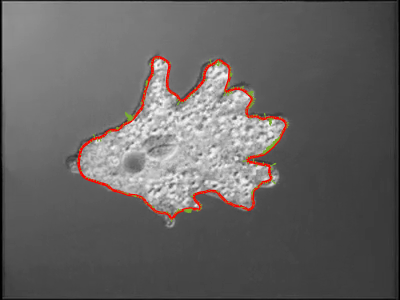
\includegraphics[width=0.45\textwidth]{./figures/defom2.png}
%	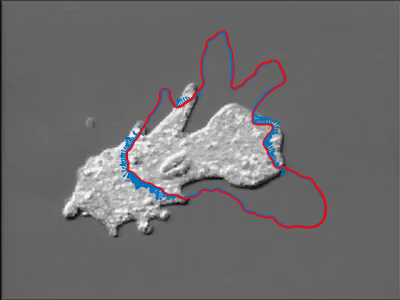
\includegraphics[width=0.45\textwidth]{./figures/defom148.png}
%	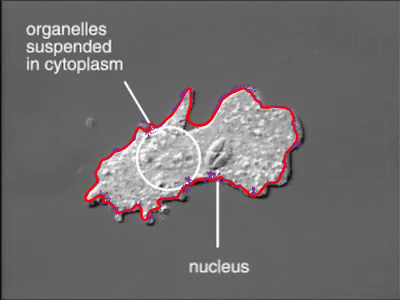
\includegraphics[width=0.45\textwidth]{./figures/defom186.png}
%	\caption{Deformable models: top-left is the initial curve, the other three shows the intermediate results.}
%\end{figure}
%	\section{Geometric Priors}
%	Several approaches have been applied for myelinated nerves segmentation, including:
%	\begin{enumerate}
%	\item Perform MRF segmentation slice by slice. This is done by firstly investigating the histogram of several sample images, and then perform MRF for binary segmentation. Parameters need to be finely tuned in order to have very good results. A snapshot of the final result is shown in Figure~\ref{final1}.
%	\begin{figure}[!b]
%	\centering
%	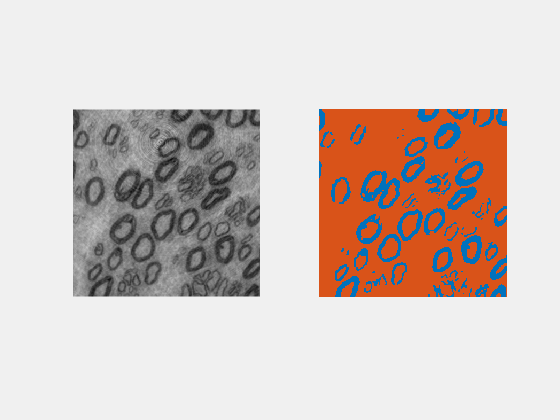
\includegraphics[width=0.8\textwidth]{./figures/1.png}
%	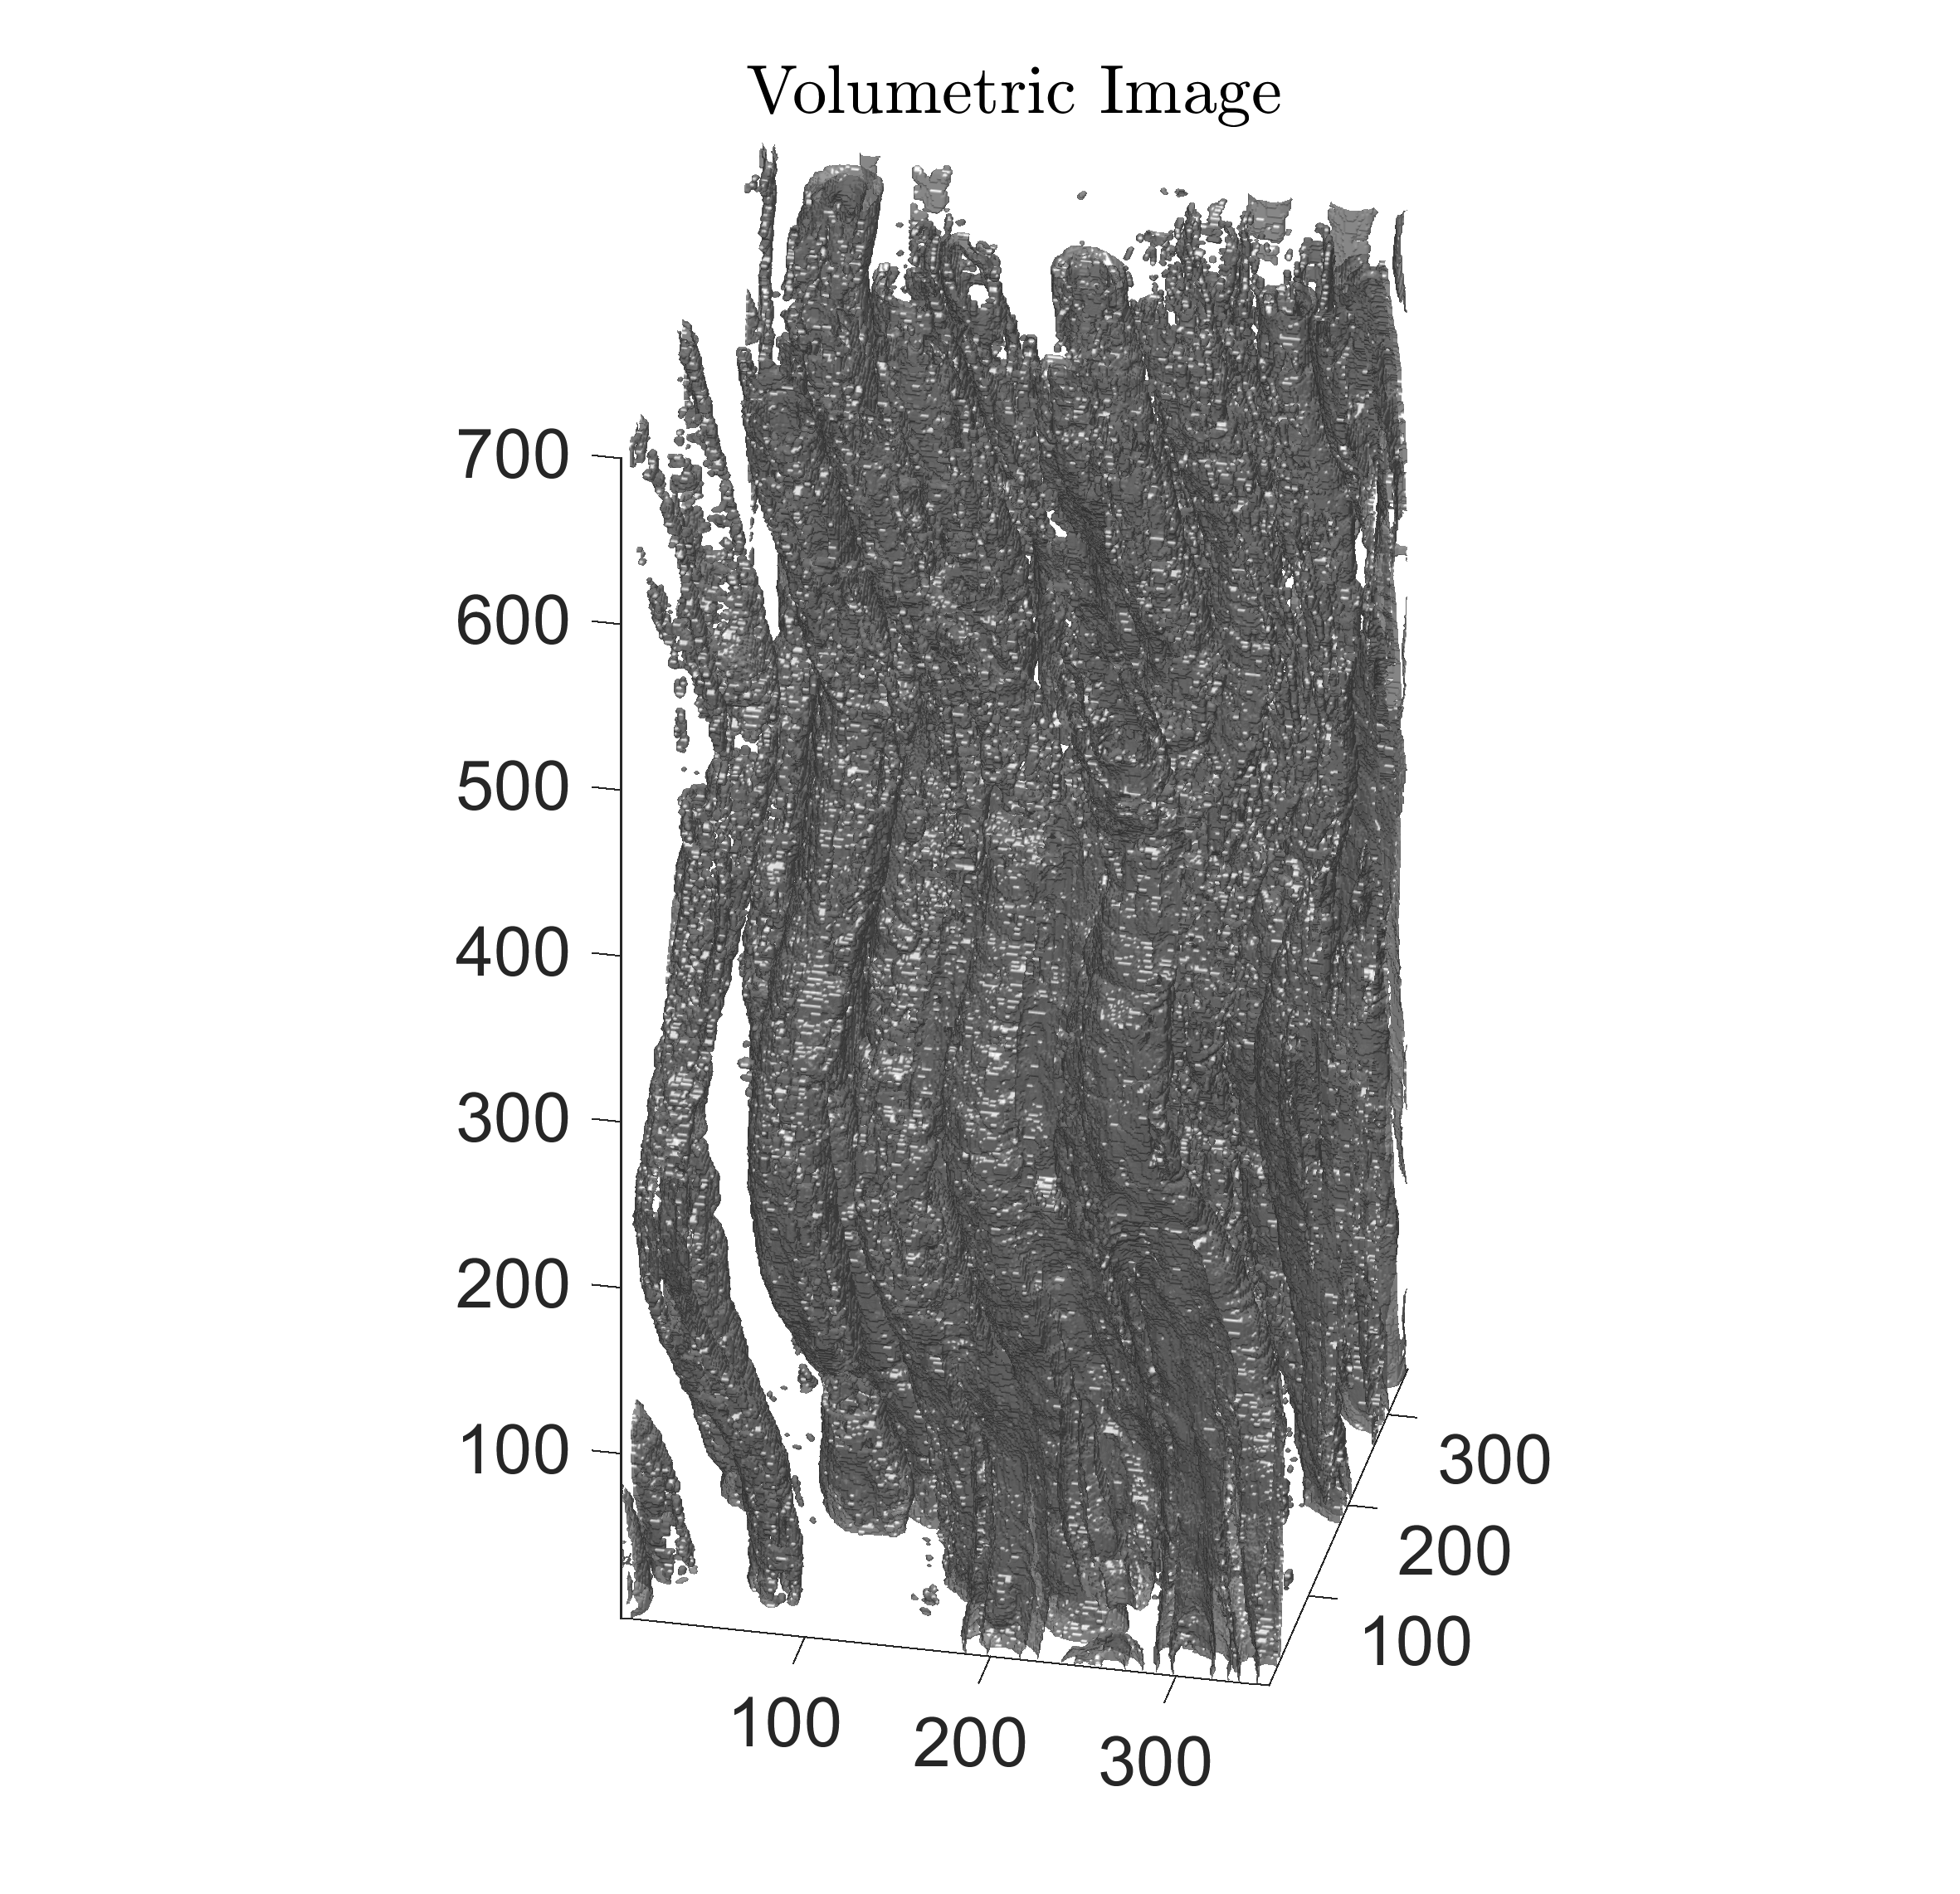
\includegraphics[width=0.8\textwidth]{./figures/final_res1.png}
%    \caption{Top image is a snapshot of the slice-by-slice MRF segmentation of nerves image. The bottom image shows the 3D visualization of the segmented nerves.}
%	\label{final1}
%\end{figure}
%	
%	\item Perform MRF by considering smoothness among consecutive frames. Theoretically, it is possible to create a full 3D segmentation by stacking all images together. However, because of the memory constraint as well as for saving time, what I did in this assignment is to do the 3D segmentation using $100$ continuous images, i.e. $1-100$ as a batch, $101-200$ as the second batch. A snapshot of the final result is shown in Figure~\ref{final2}.
%	
%	\begin{figure}[!b]
%	\centering
%	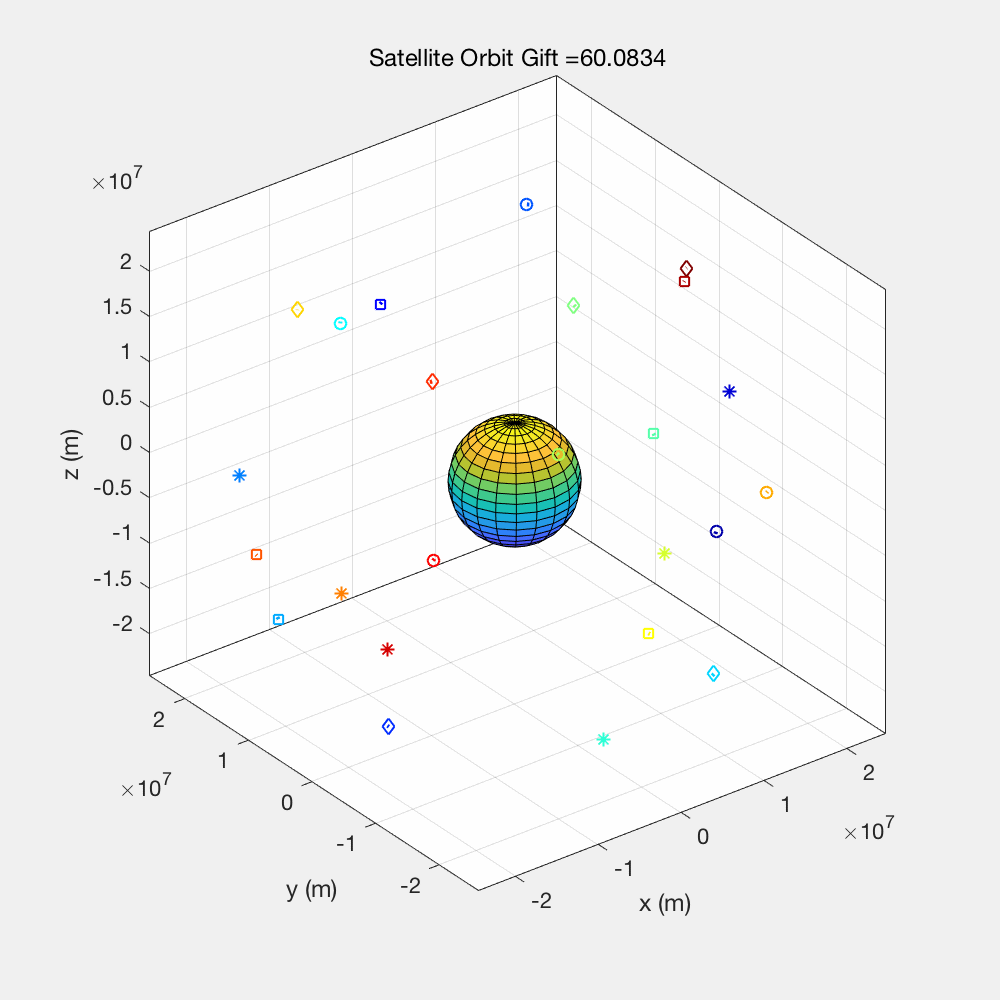
\includegraphics[width=0.8\textwidth]{./figures/2.png}
%	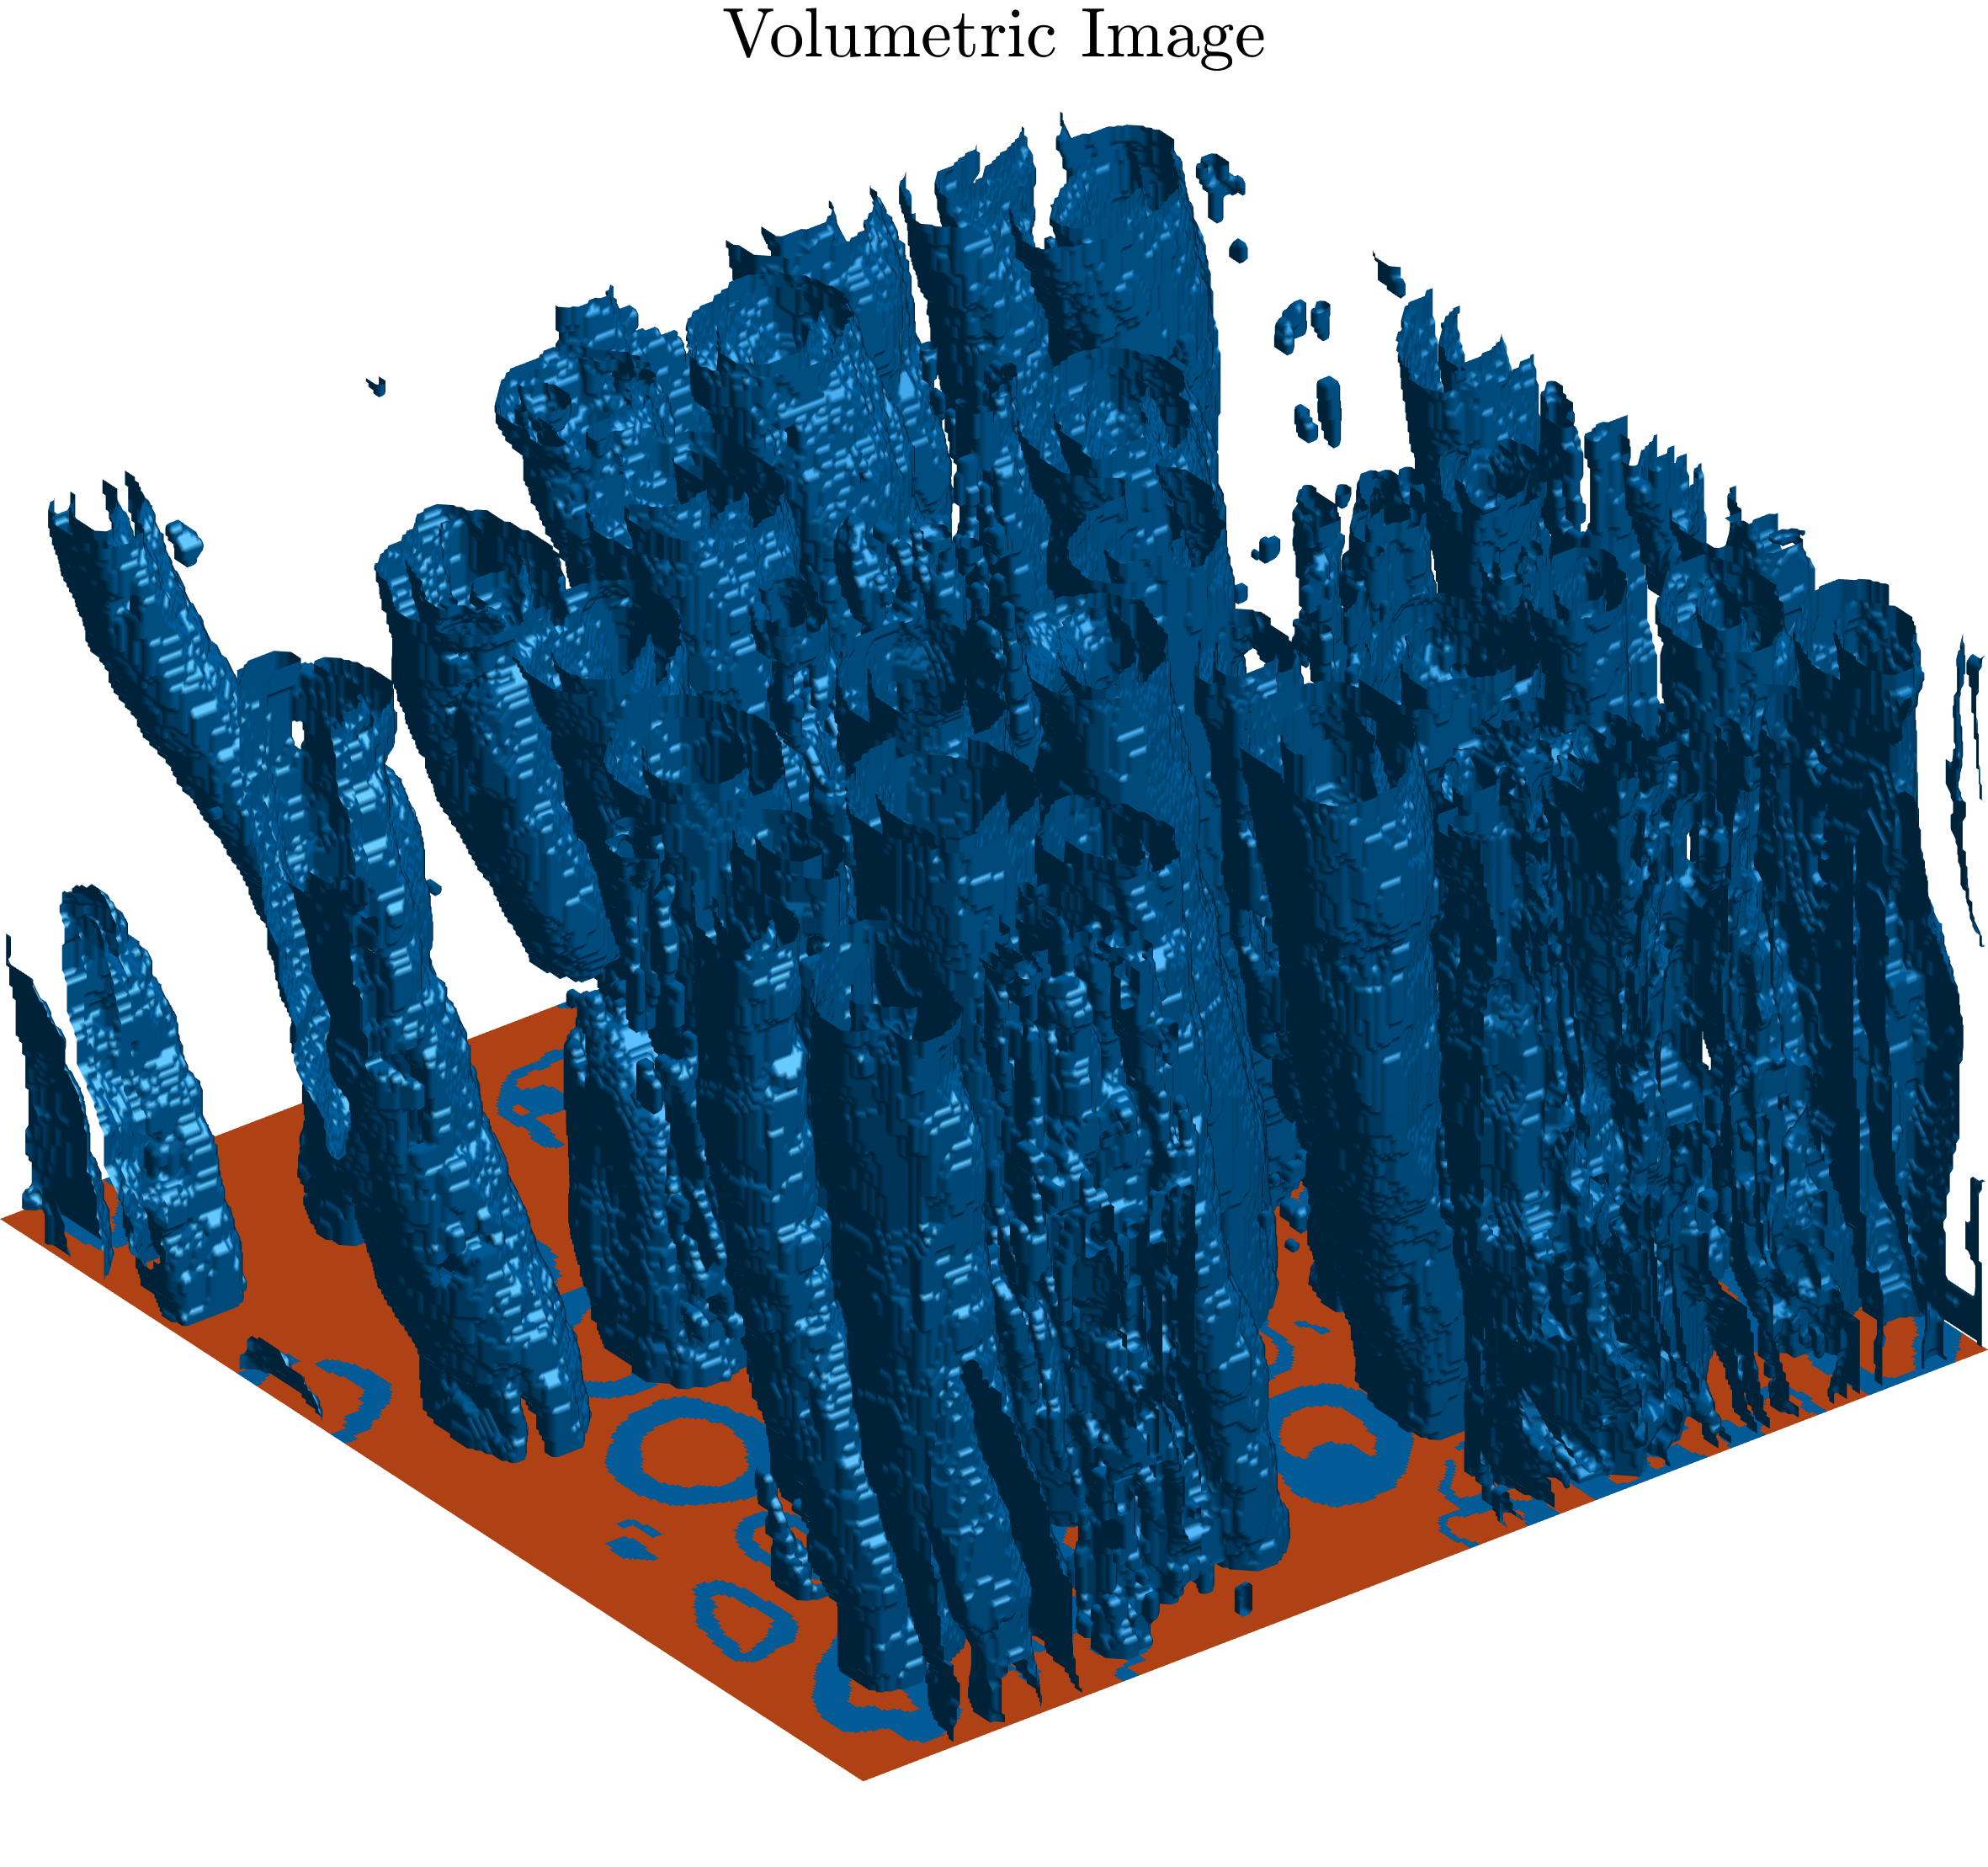
\includegraphics[width=0.8\textwidth]{./figures/final_res2.png}
%    \caption{Top image is a snapshot of the $3$D MRF segmentation of nerves image. Bottom image shows the 3D visualization of the segmented nerves (using $1-300$ frames).}
%\label{final2}
%\end{figure}    
	



	
%https://youtu.be/KMWywGcNNjI	
%https://youtu.be/_GslxUDEZzM
	
	%\bibliography{PnPCites} 
	%\bibliographystyle{ieeetr}
	
\end{document}